% !TEX root = ../proyect.tex


\chapter{Relación de endpoints de la API}\label{apendice-endpoints}

Todos los endpoints cuelgan del prefijo \texttt{/api/v1/} y, salvo indicación contraria,
requieren autenticación JWT. La especificación OpenAPI completa se publica en
\texttt{/api/v1/schema/} (con interfaces Swagger UI y ReDoc).

\begin{small}
\begin{longtable}{@{}llp{6.4cm}@{}}
\caption{Endpoints de la API por módulo}\label{tab:endpoints-completos}\\
\toprule
\textbf{Método} & \textbf{Ruta} & \textbf{Descripción} \\
\midrule
\endfirsthead
\toprule
\textbf{Método} & \textbf{Ruta} & \textbf{Descripción} \\
\midrule
\endhead
\bottomrule
\endfoot
GET & \texttt{health/} & Health check público (exento de throttling) \\
\midrule
POST & \texttt{auth/register/} & Registro de usuario (público) \\
POST & \texttt{auth/token/} & Obtención de tokens JWT (público) \\
POST & \texttt{auth/token/refresh/} & Renovación del token de acceso \\
POST & \texttt{auth/password-reset/} & Solicitud de restablecimiento (público) \\
POST & \texttt{auth/password-reset/confirm/} & Confirmación de restablecimiento \\
GET/PATCH & \texttt{auth/profile/} & Perfil y preferencias del usuario \\
\midrule
GET & \texttt{products/} & Listado y búsqueda fuzzy de productos \\
GET & \texttt{products/\{id\}/} & Detalle de producto \\
GET & \texttt{products/categories/} & Jerarquía de categorías \\
POST & \texttt{products/proposals/} & Propuesta de alta de un nuevo producto \\
* & \texttt{products/proposals/admin/} & Moderación de propuestas (administrador) \\
\midrule
GET & \texttt{stores/} & Búsqueda geoespacial (\texttt{lat}, \texttt{lng}, \texttt{radius\_km}) o favoritas \\
GET & \texttt{stores/\{id\}/} & Detalle de tienda \\
POST & \texttt{stores/\{id\}/favorite/} & Alternar tienda favorita \\
\midrule
POST & \texttt{prices/compare/} & Comparativa de un producto entre tiendas \\
POST & \texttt{prices/list-total/} & Coste total de una lista por tienda \\
GET & \texttt{prices/\{product\_id\}/history/} & Histórico de precios \\
* & \texttt{prices/alerts/} & CRUD de alertas de precio \\
\midrule
* & \texttt{lists/} & CRUD de listas de la compra e ítems \\
* & \texttt{lists/templates/} & CRUD de plantillas de lista \\
\midrule
POST & \texttt{optimize/} & Calcular o recalcular la ruta óptima \\
GET & \texttt{optimize/?shopping\_list\_id=\{id\}} & Última ruta persistida de una lista \\
POST & \texttt{optimize/choices/} & Resolución de ambigüedad semántica y recálculo \\
\midrule
POST & \texttt{ocr/scan/} & Procesado OCR de imagen (límite 60/h) \\
\midrule
POST & \texttt{assistant/chat/} & Mensaje al asistente LLM (límite 30/h) \\
\midrule
* & \texttt{business/profiles/} & Alta y gestión de perfiles PYME, con acciones de aprobación y rechazo para administradores \\
* & \texttt{business/prices/} & Gestión de precios del comercio (incl. carga CSV) \\
* & \texttt{business/promotions/} & Gestión de promociones \\
\midrule
* & \texttt{notifications/} & Buzón de notificaciones (lectura, borrado lógico) \\
POST & \texttt{notifications/push-token/} & Registro del token push del dispositivo \\
\end{longtable}
\end{small}

Las filas marcadas con * corresponden a \emph{routers} DRF que exponen el conjunto estándar de
operaciones (GET de colección y detalle, POST, PATCH, DELETE) más las acciones espec\'ificas
indicadas.

\clearpage

\chapter{Capturas de la versión de escritorio}\label{apendice-capturas-web}

Este apéndice complementa la Sección~\ref{sec:manual-web} con las capturas restantes de la
aplicación de usuario ejecutada en navegador de escritorio (ventana de 1440$\times$900).

\begin{figure}[htbp]
\centering
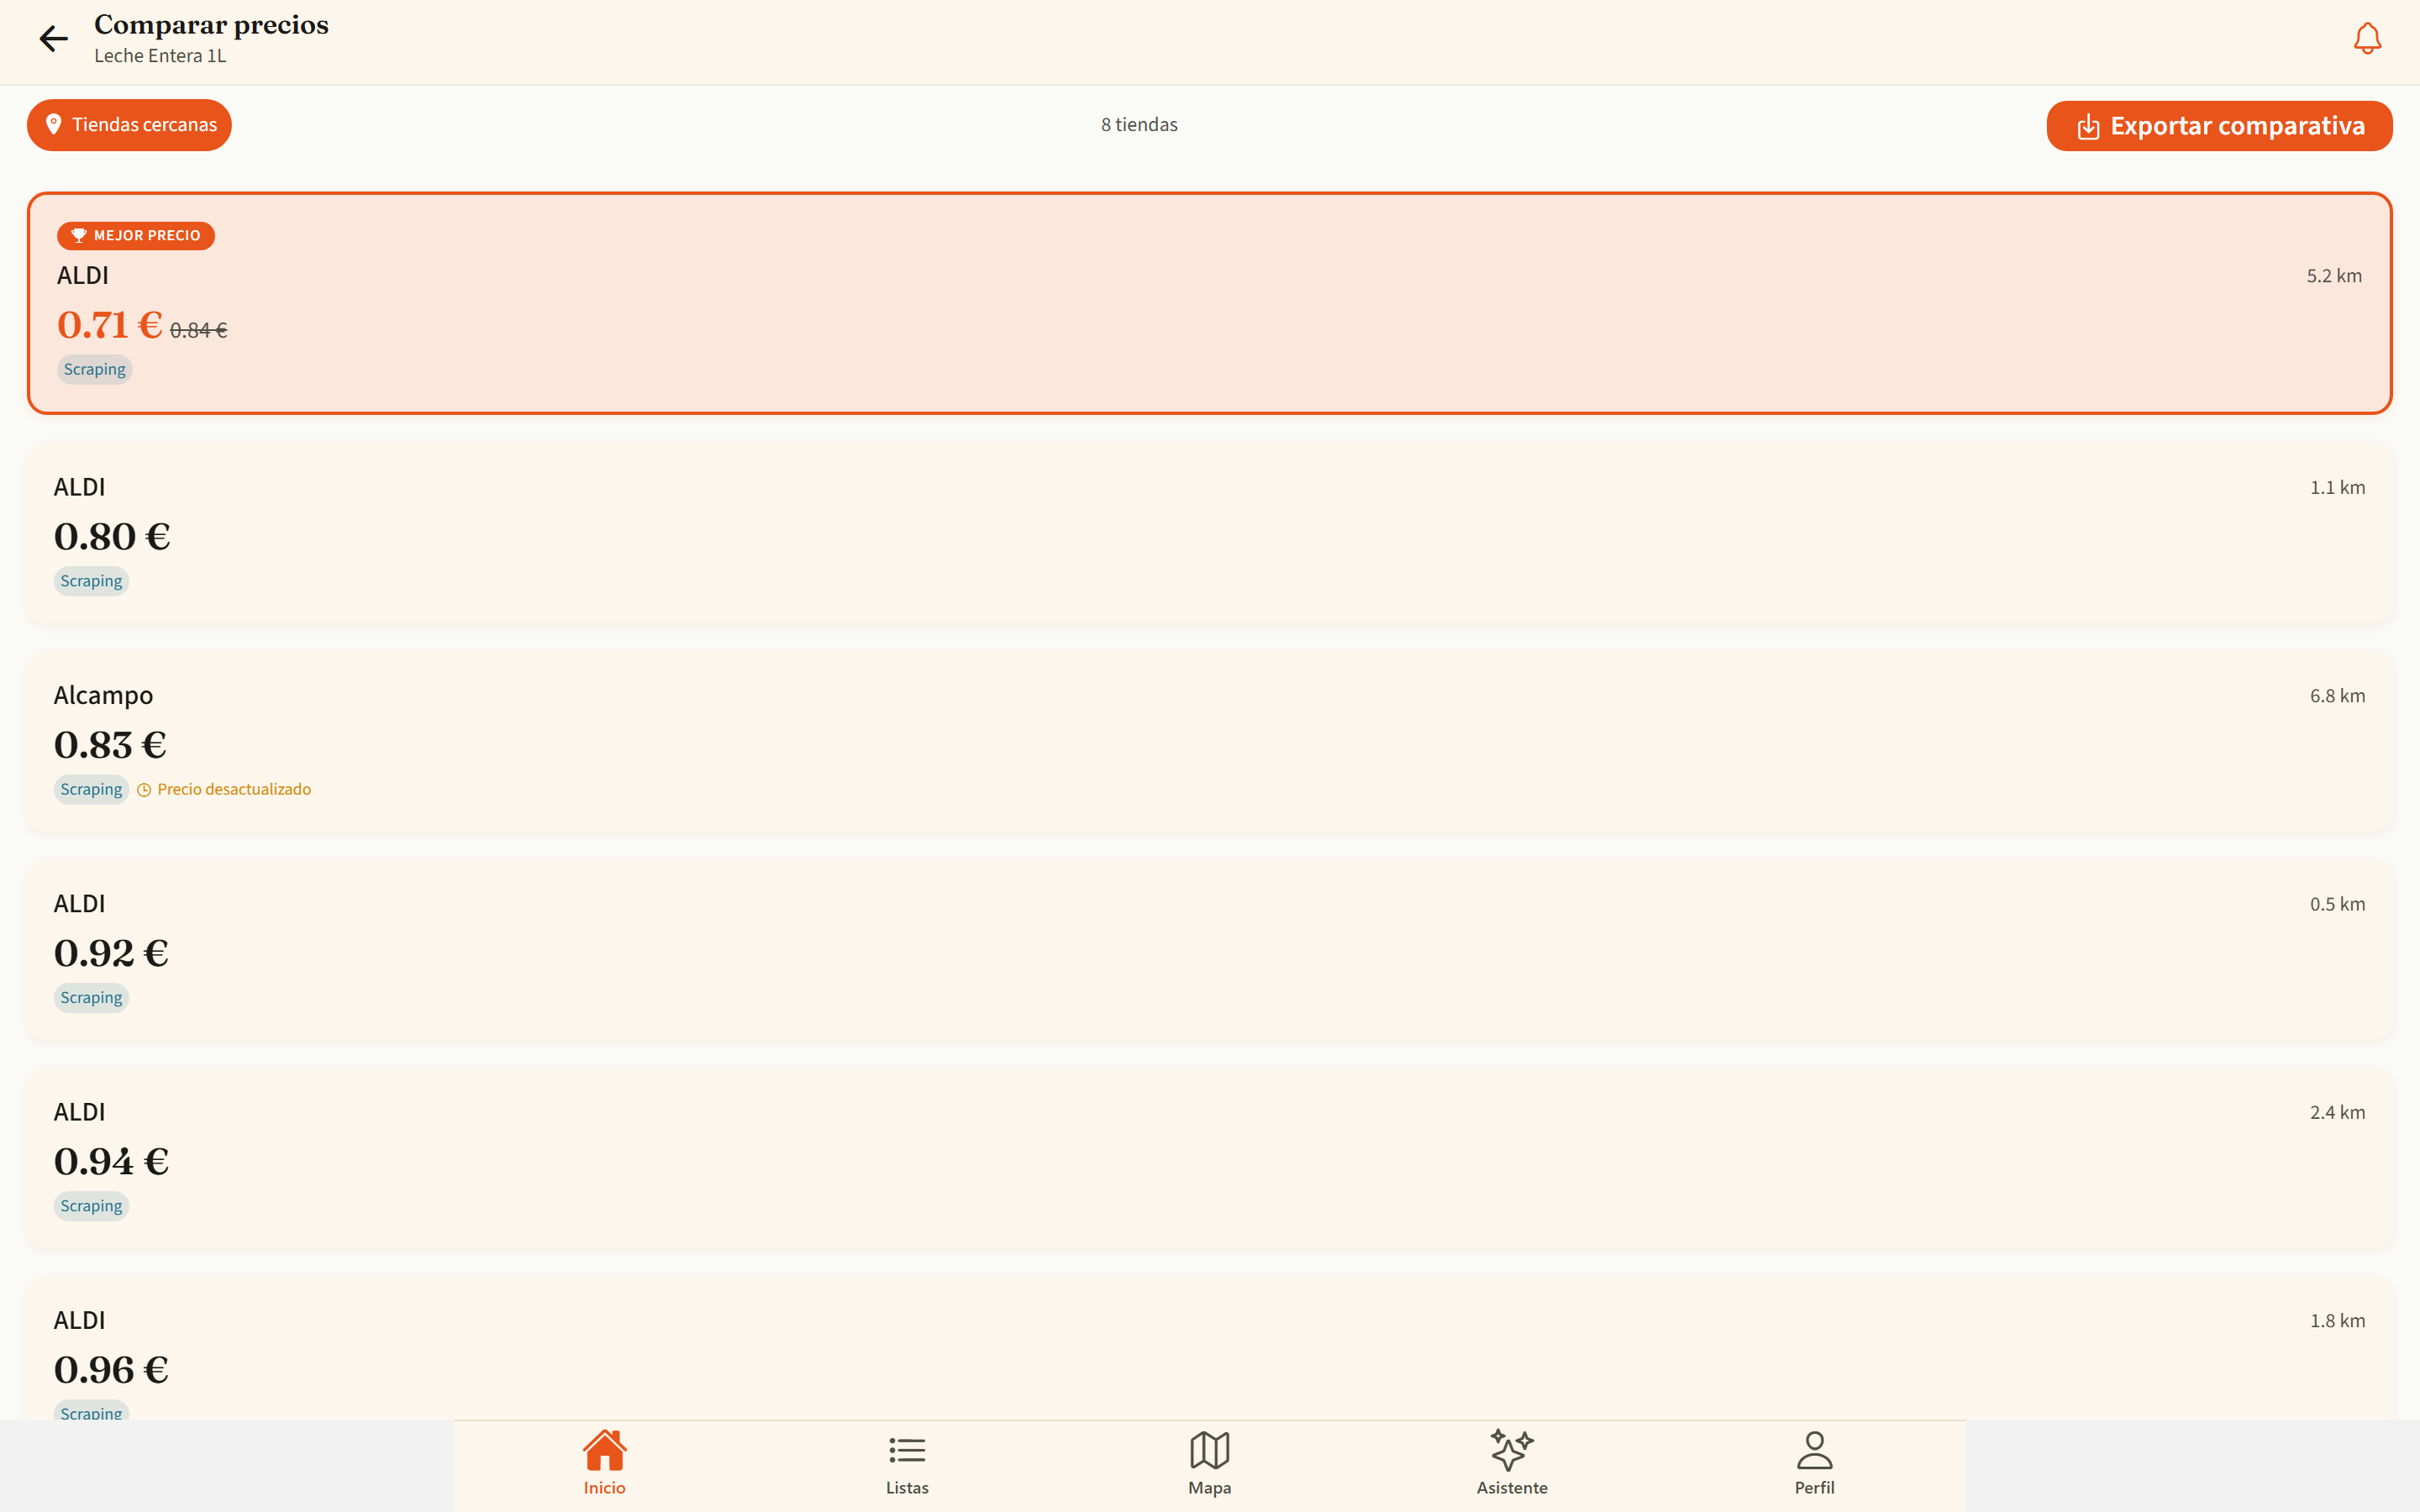
\includegraphics[width=0.48\textwidth]{diagramas/capturas/web-comparativa.png}
\hfill
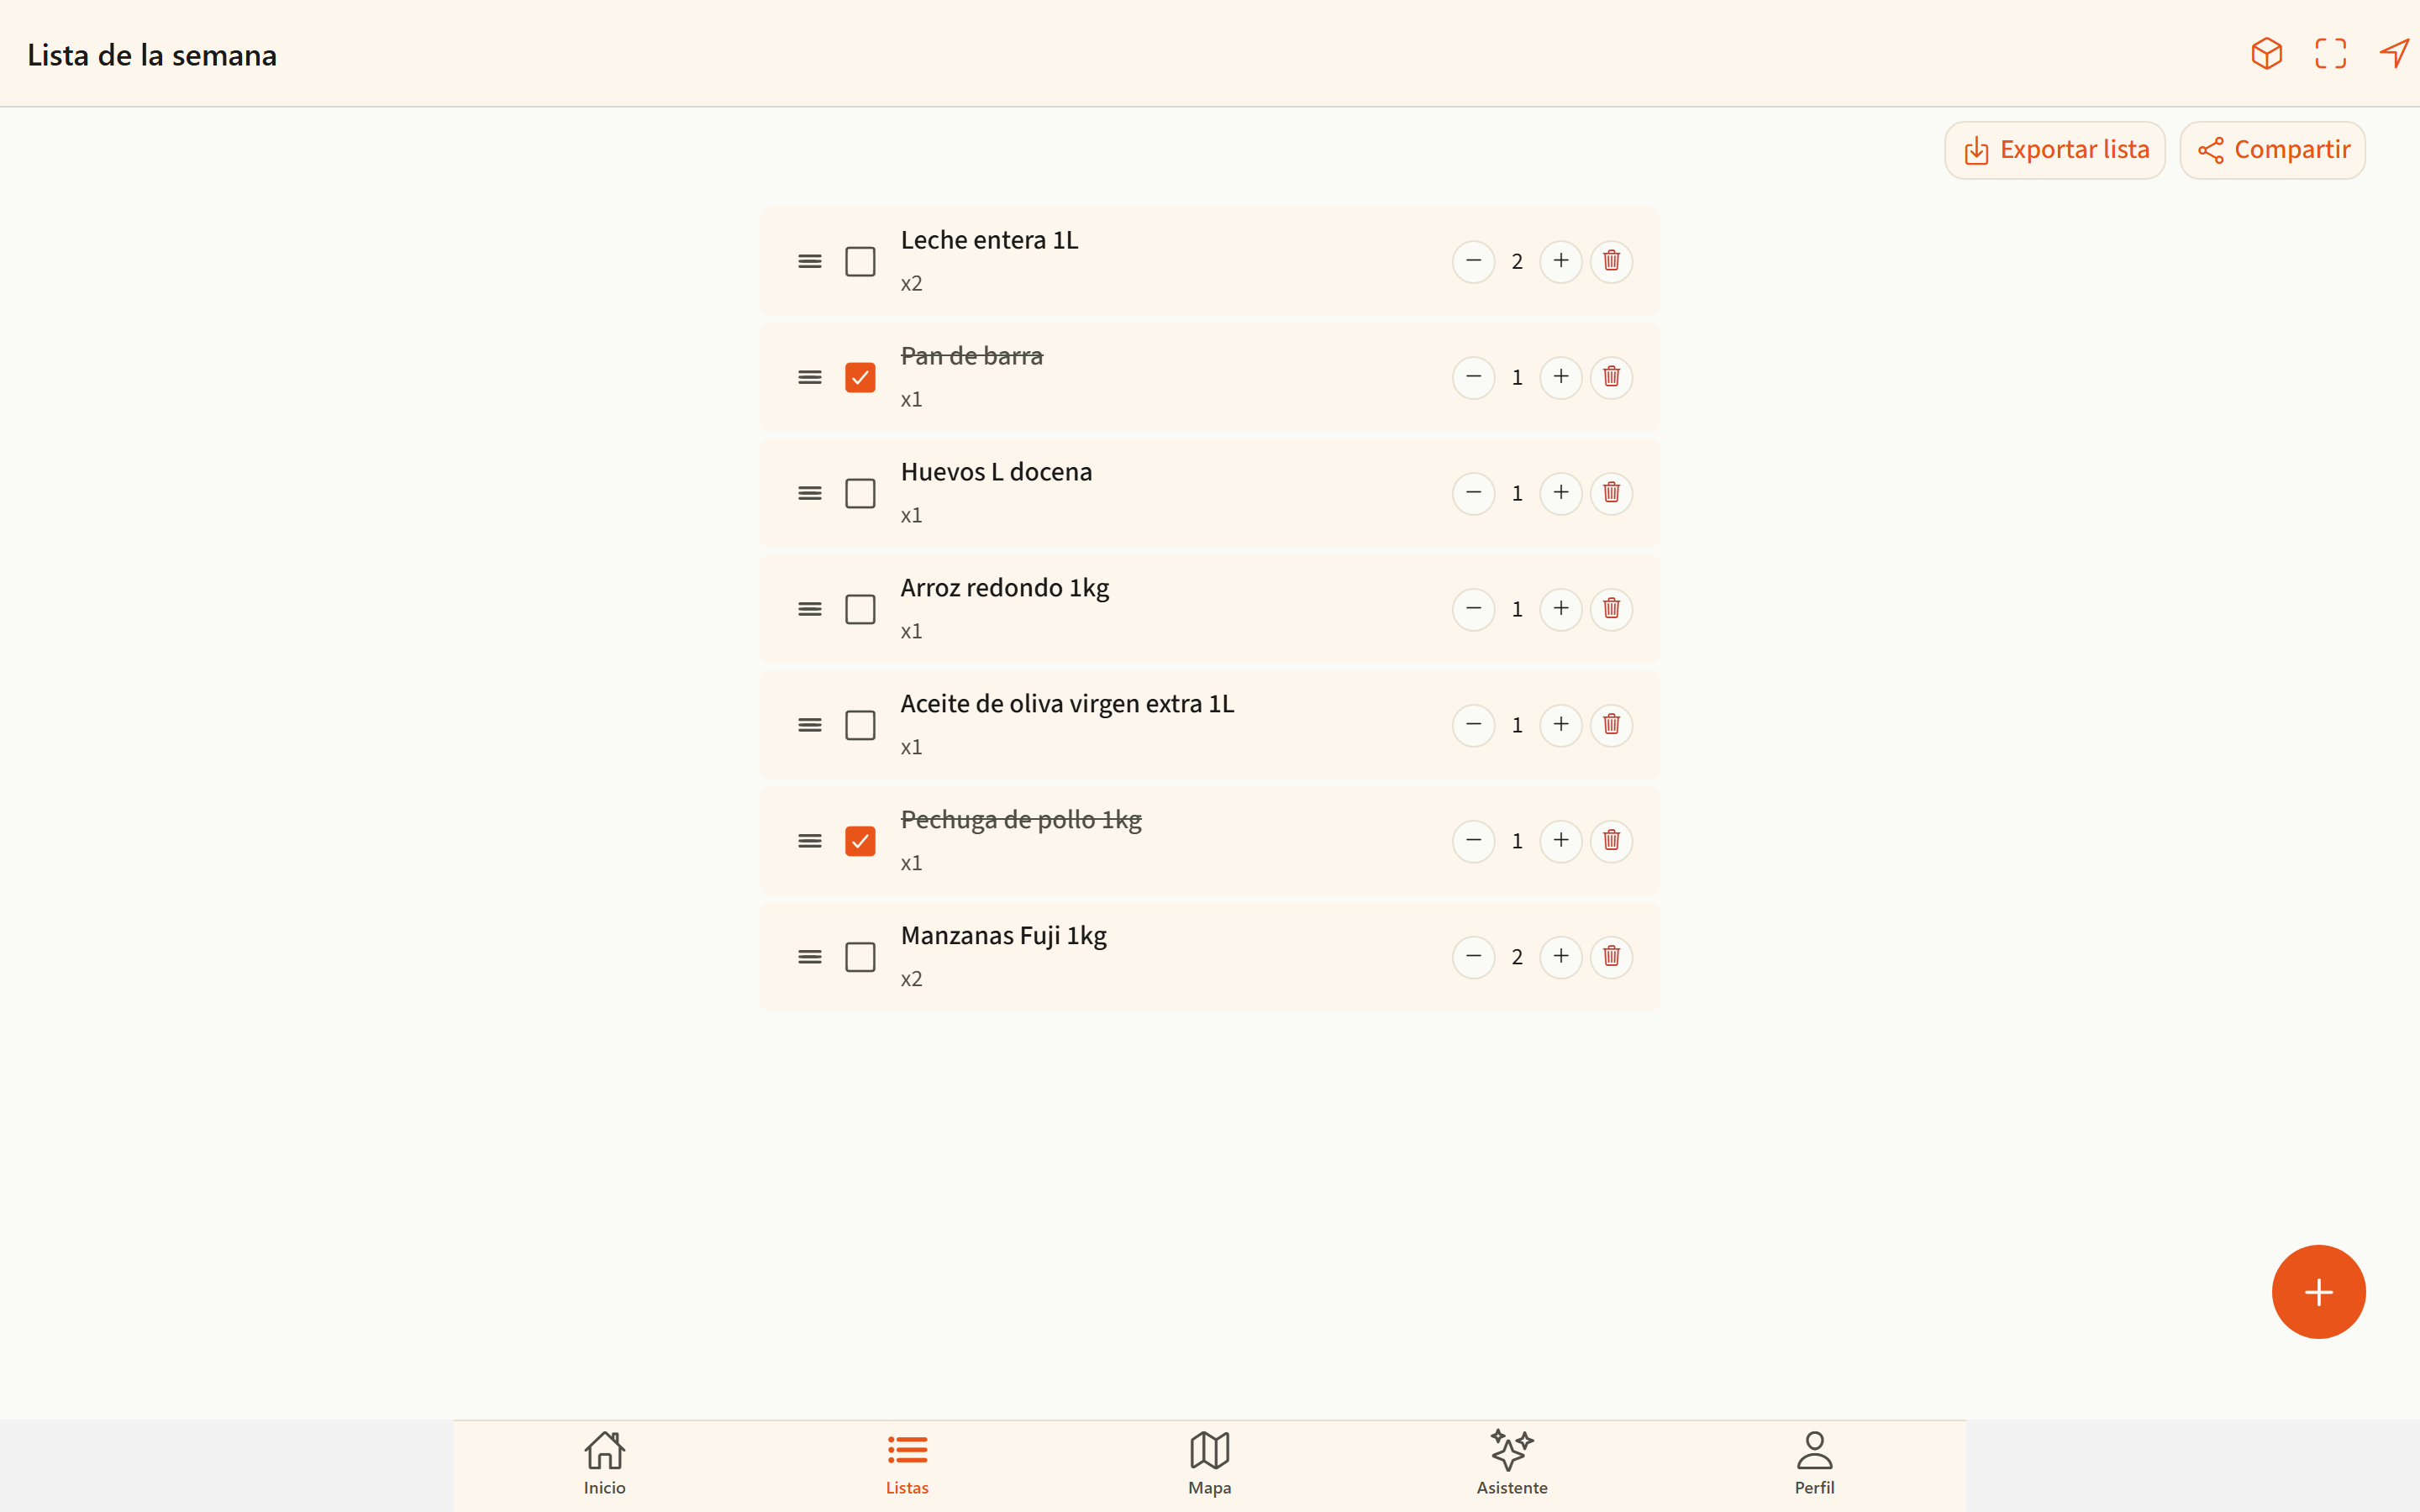
\includegraphics[width=0.48\textwidth]{diagramas/capturas/web-lista-detalle.png}
\caption{Comparativa de precios con cabecera fija y exportación CSV (izquierda) y detalle de
lista con reordenado por arrastre y exportación (derecha)}
\label{fig:manual-web-comparativa}
\end{figure}

\begin{figure}[htbp]
\centering
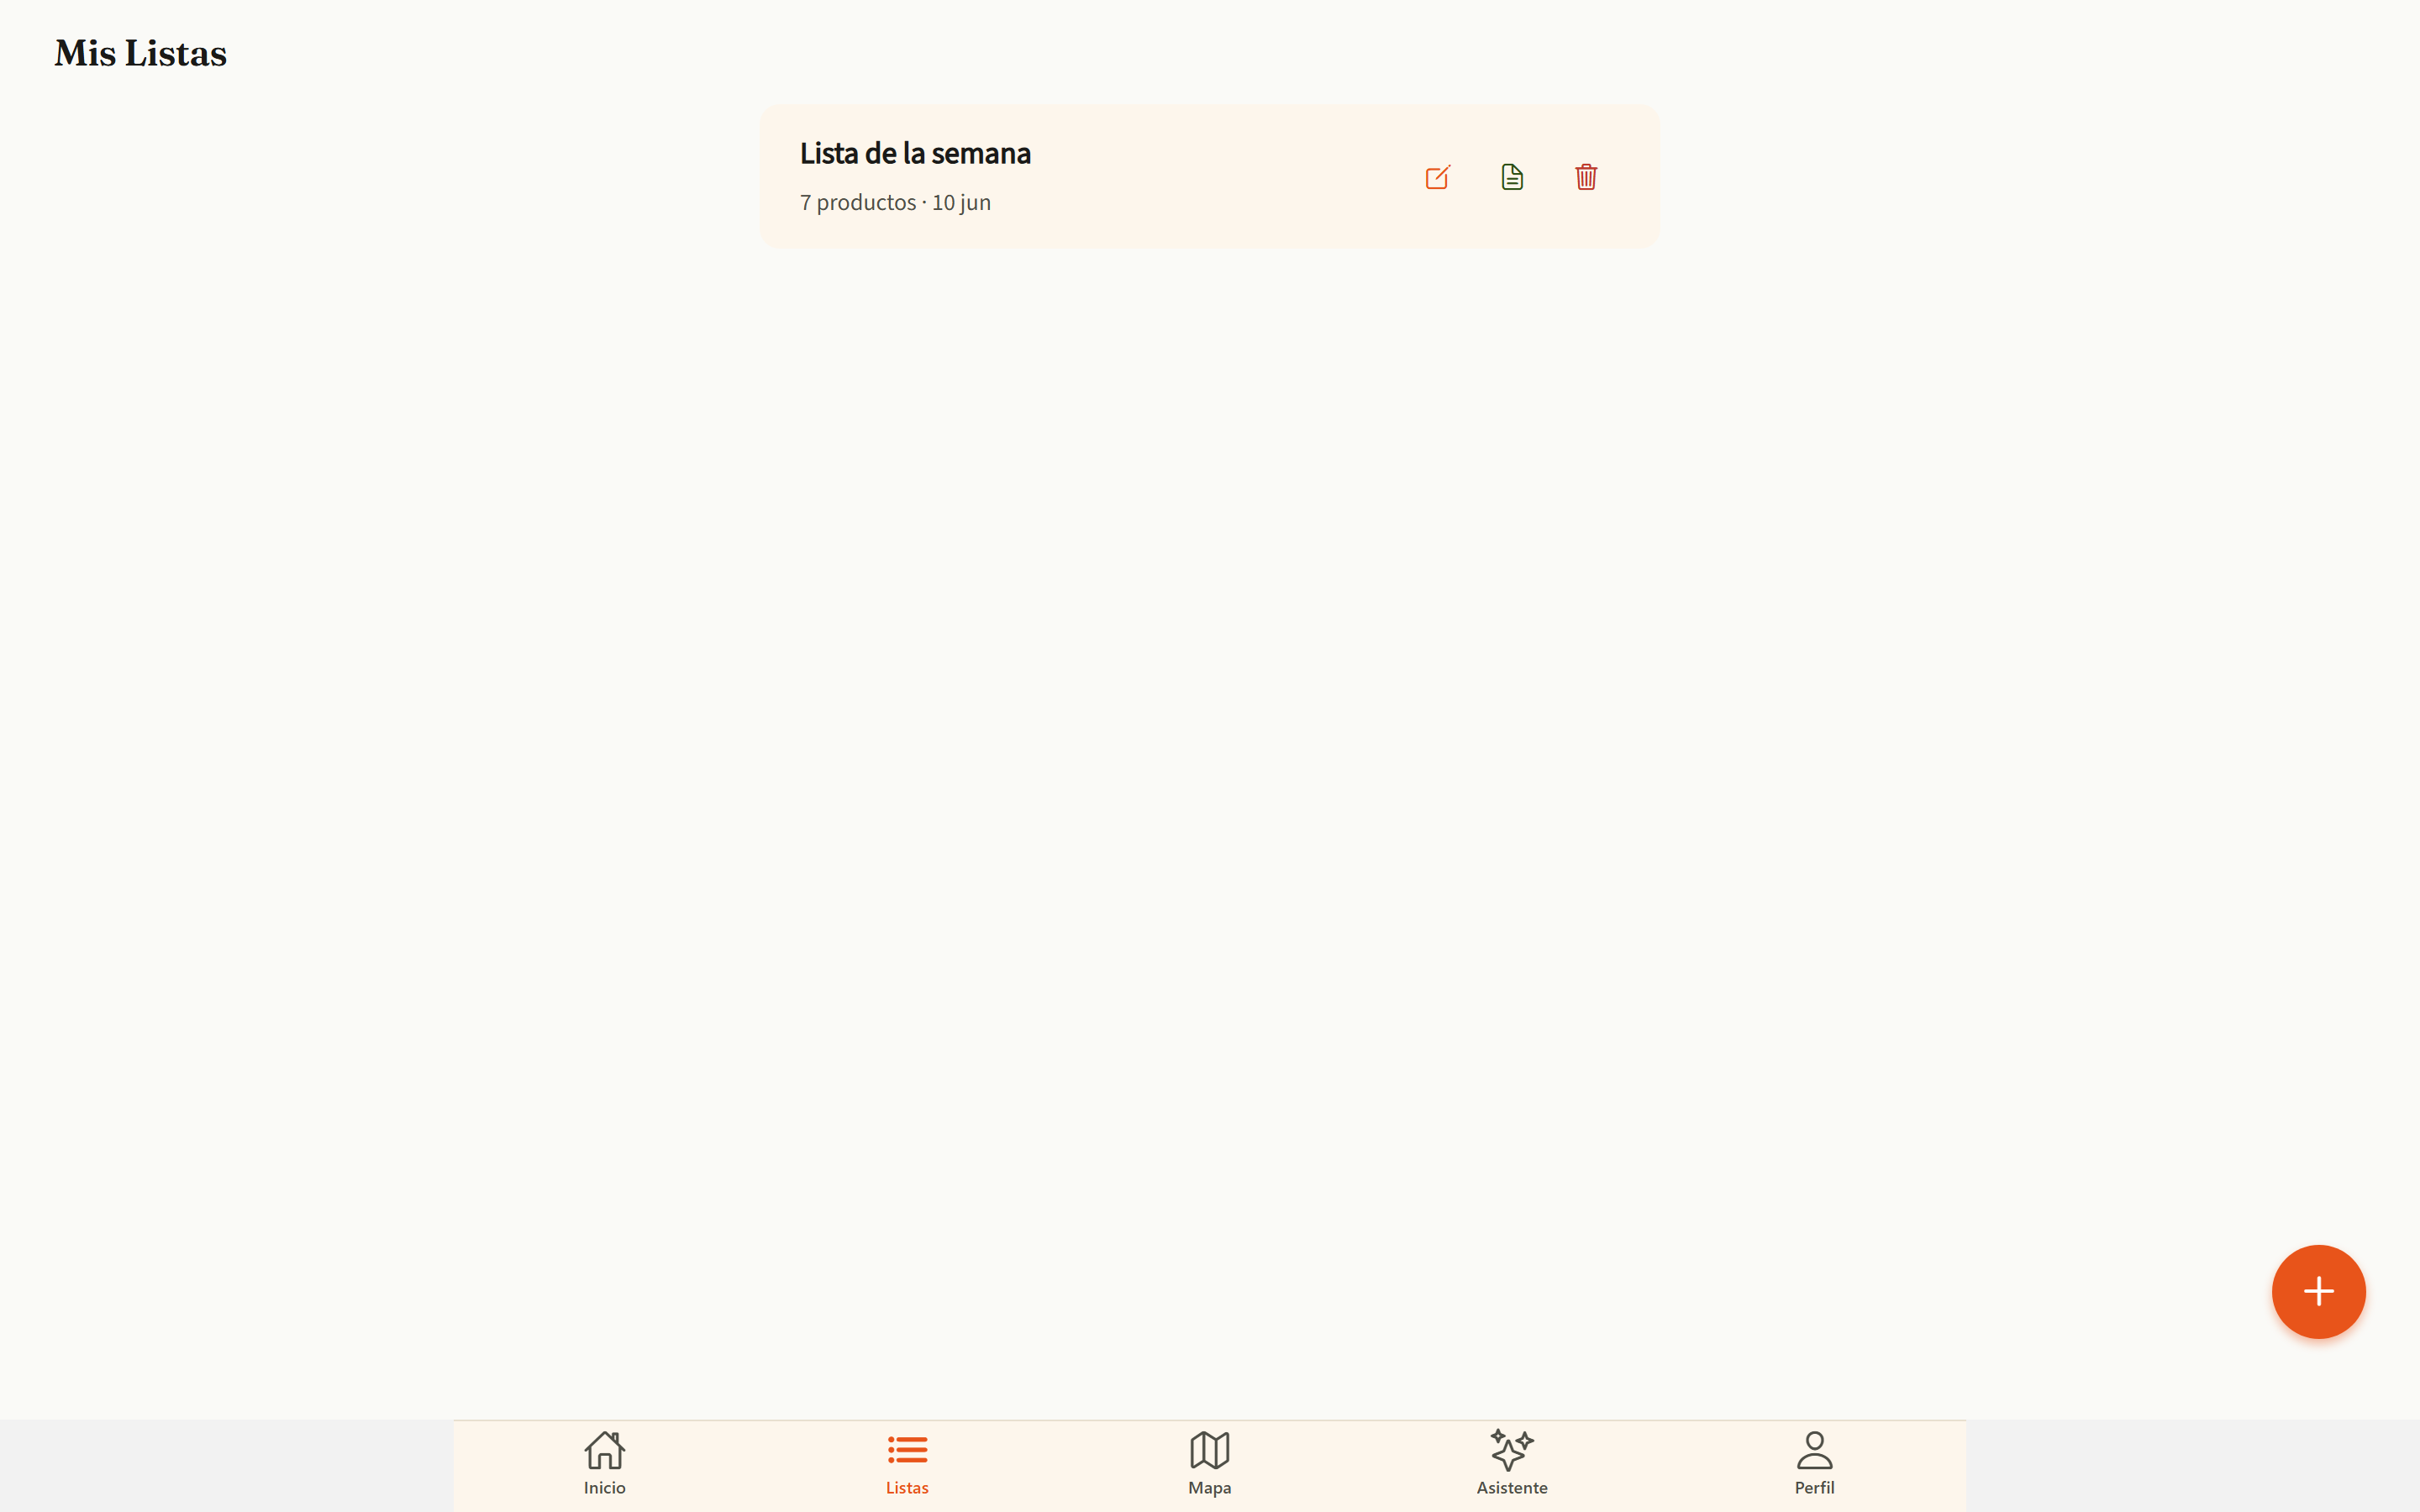
\includegraphics[width=0.48\textwidth]{diagramas/capturas/web-listas.png}
\hfill
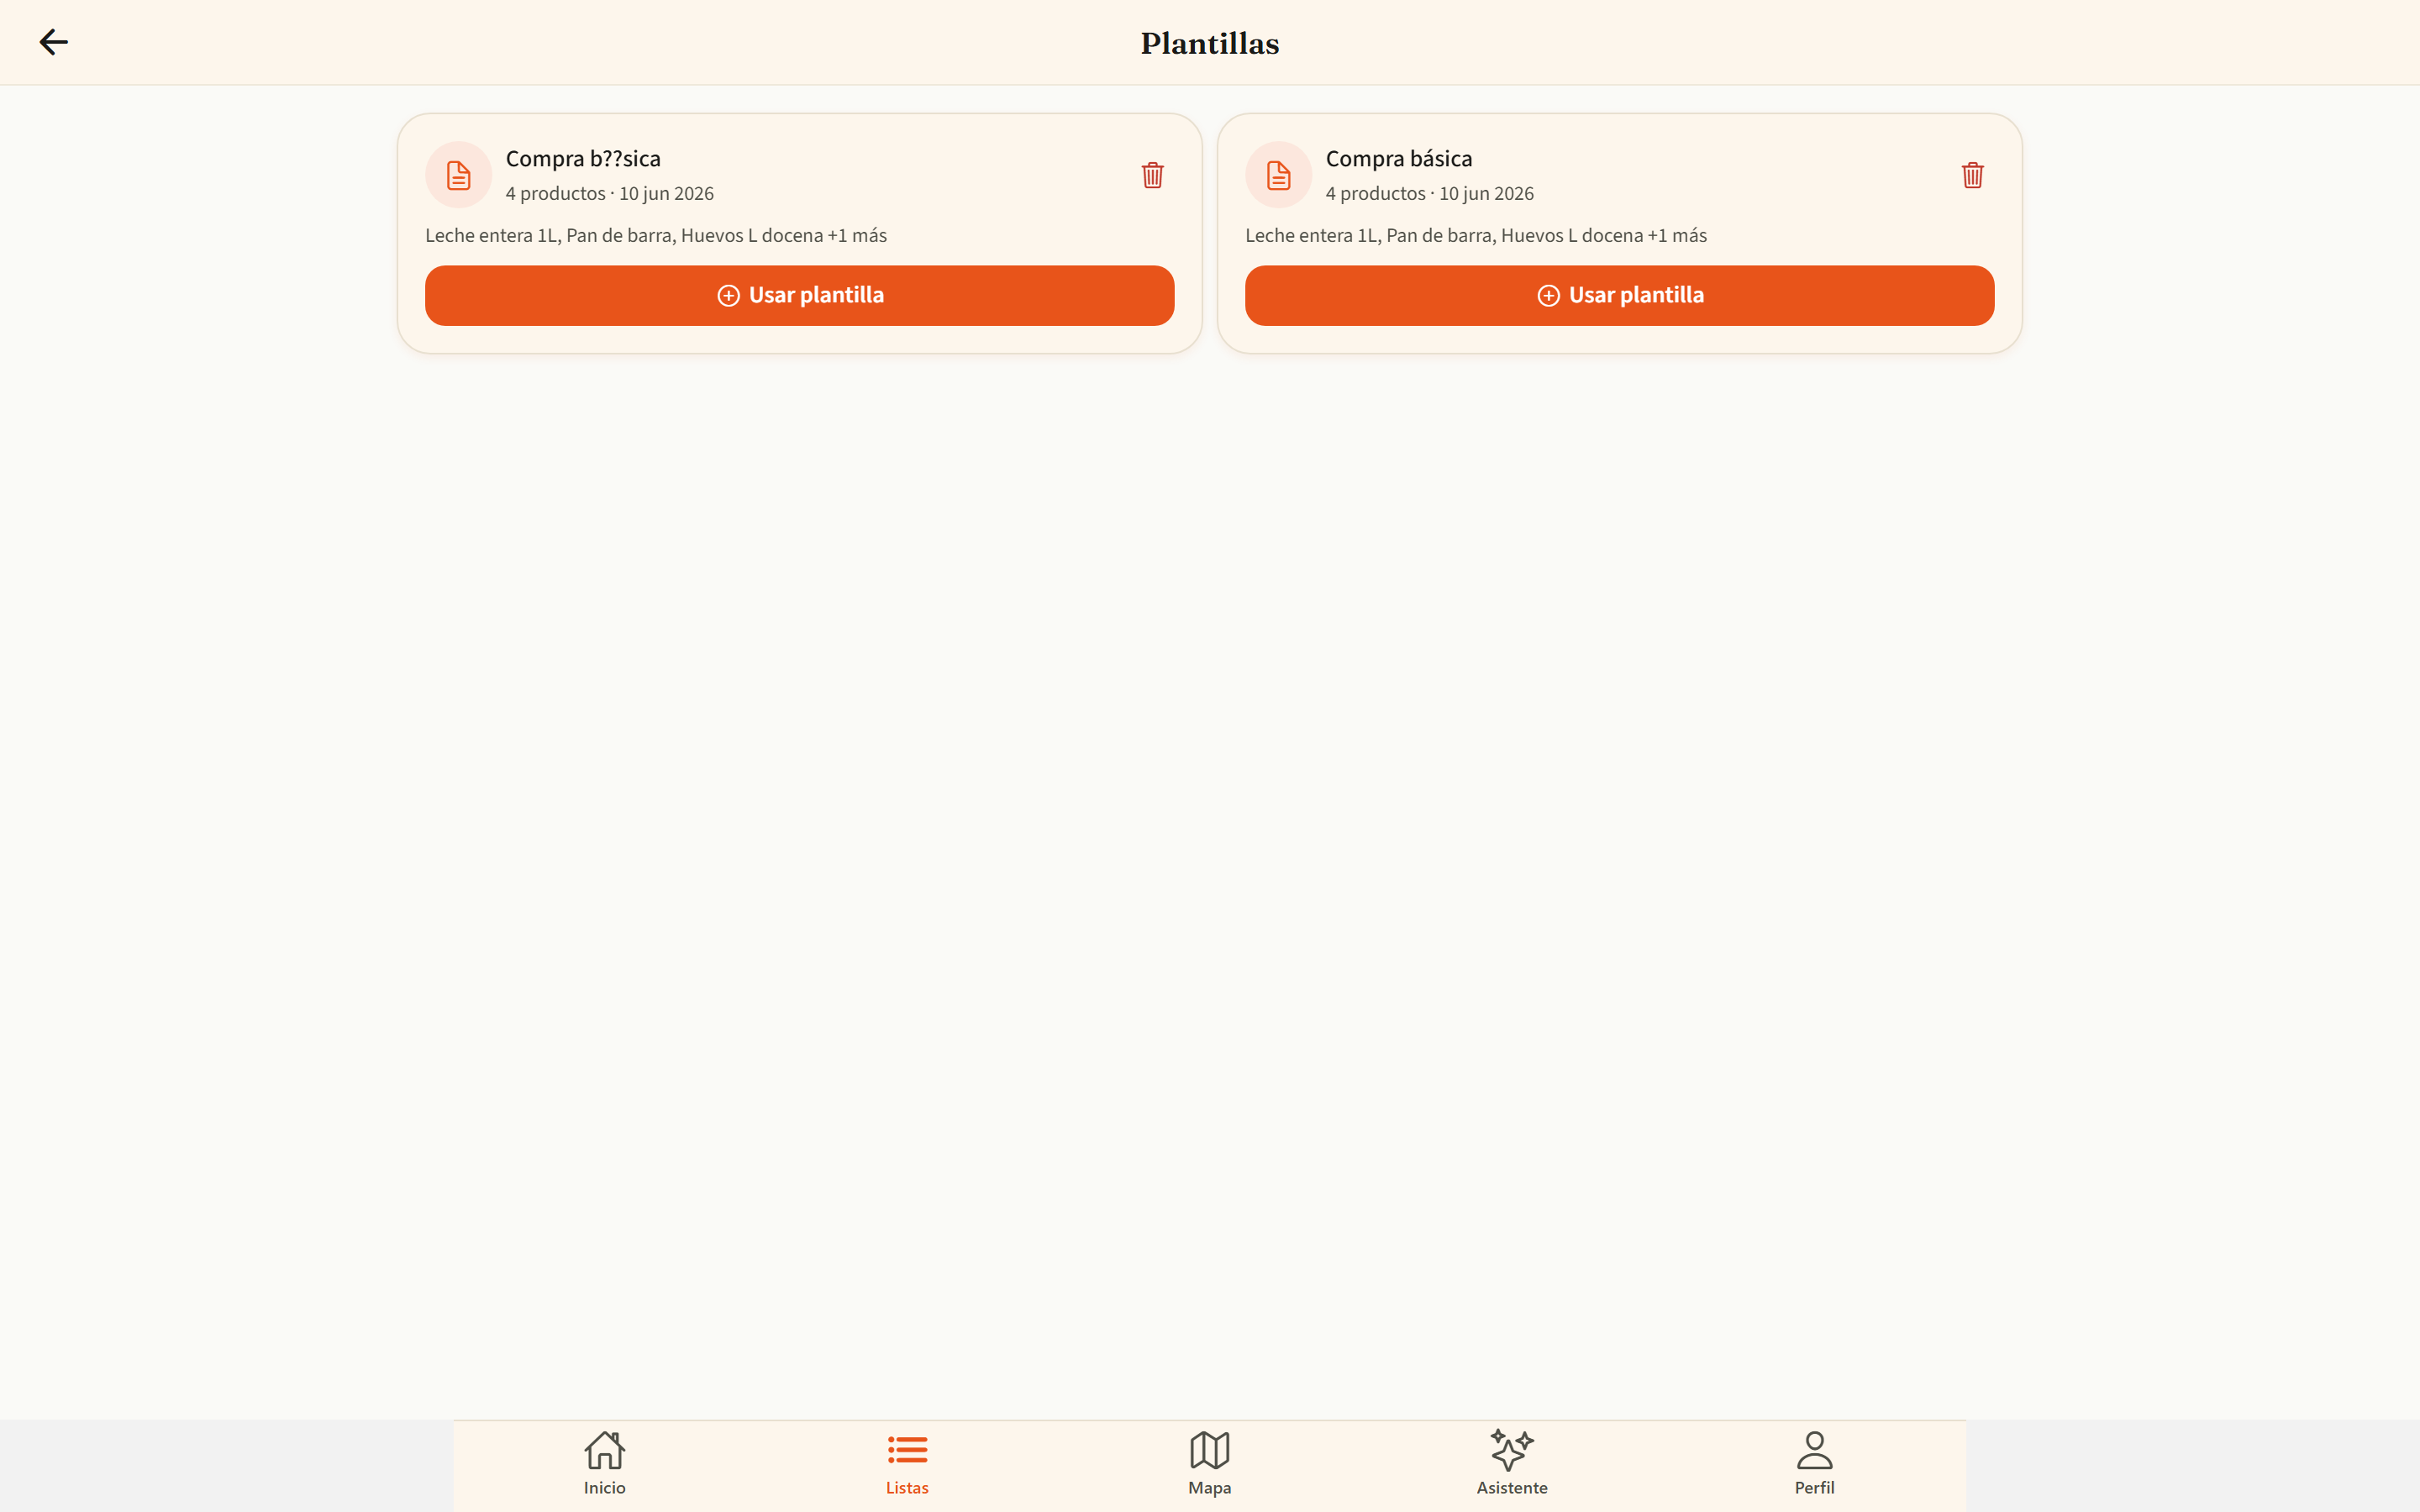
\includegraphics[width=0.48\textwidth]{diagramas/capturas/web-plantillas.png}
\caption{Colecciones en rejilla responsiva: listas de la compra (izquierda) y plantillas
(derecha)}
\label{fig:manual-web-listas}
\end{figure}

\begin{figure}[htbp]
\centering
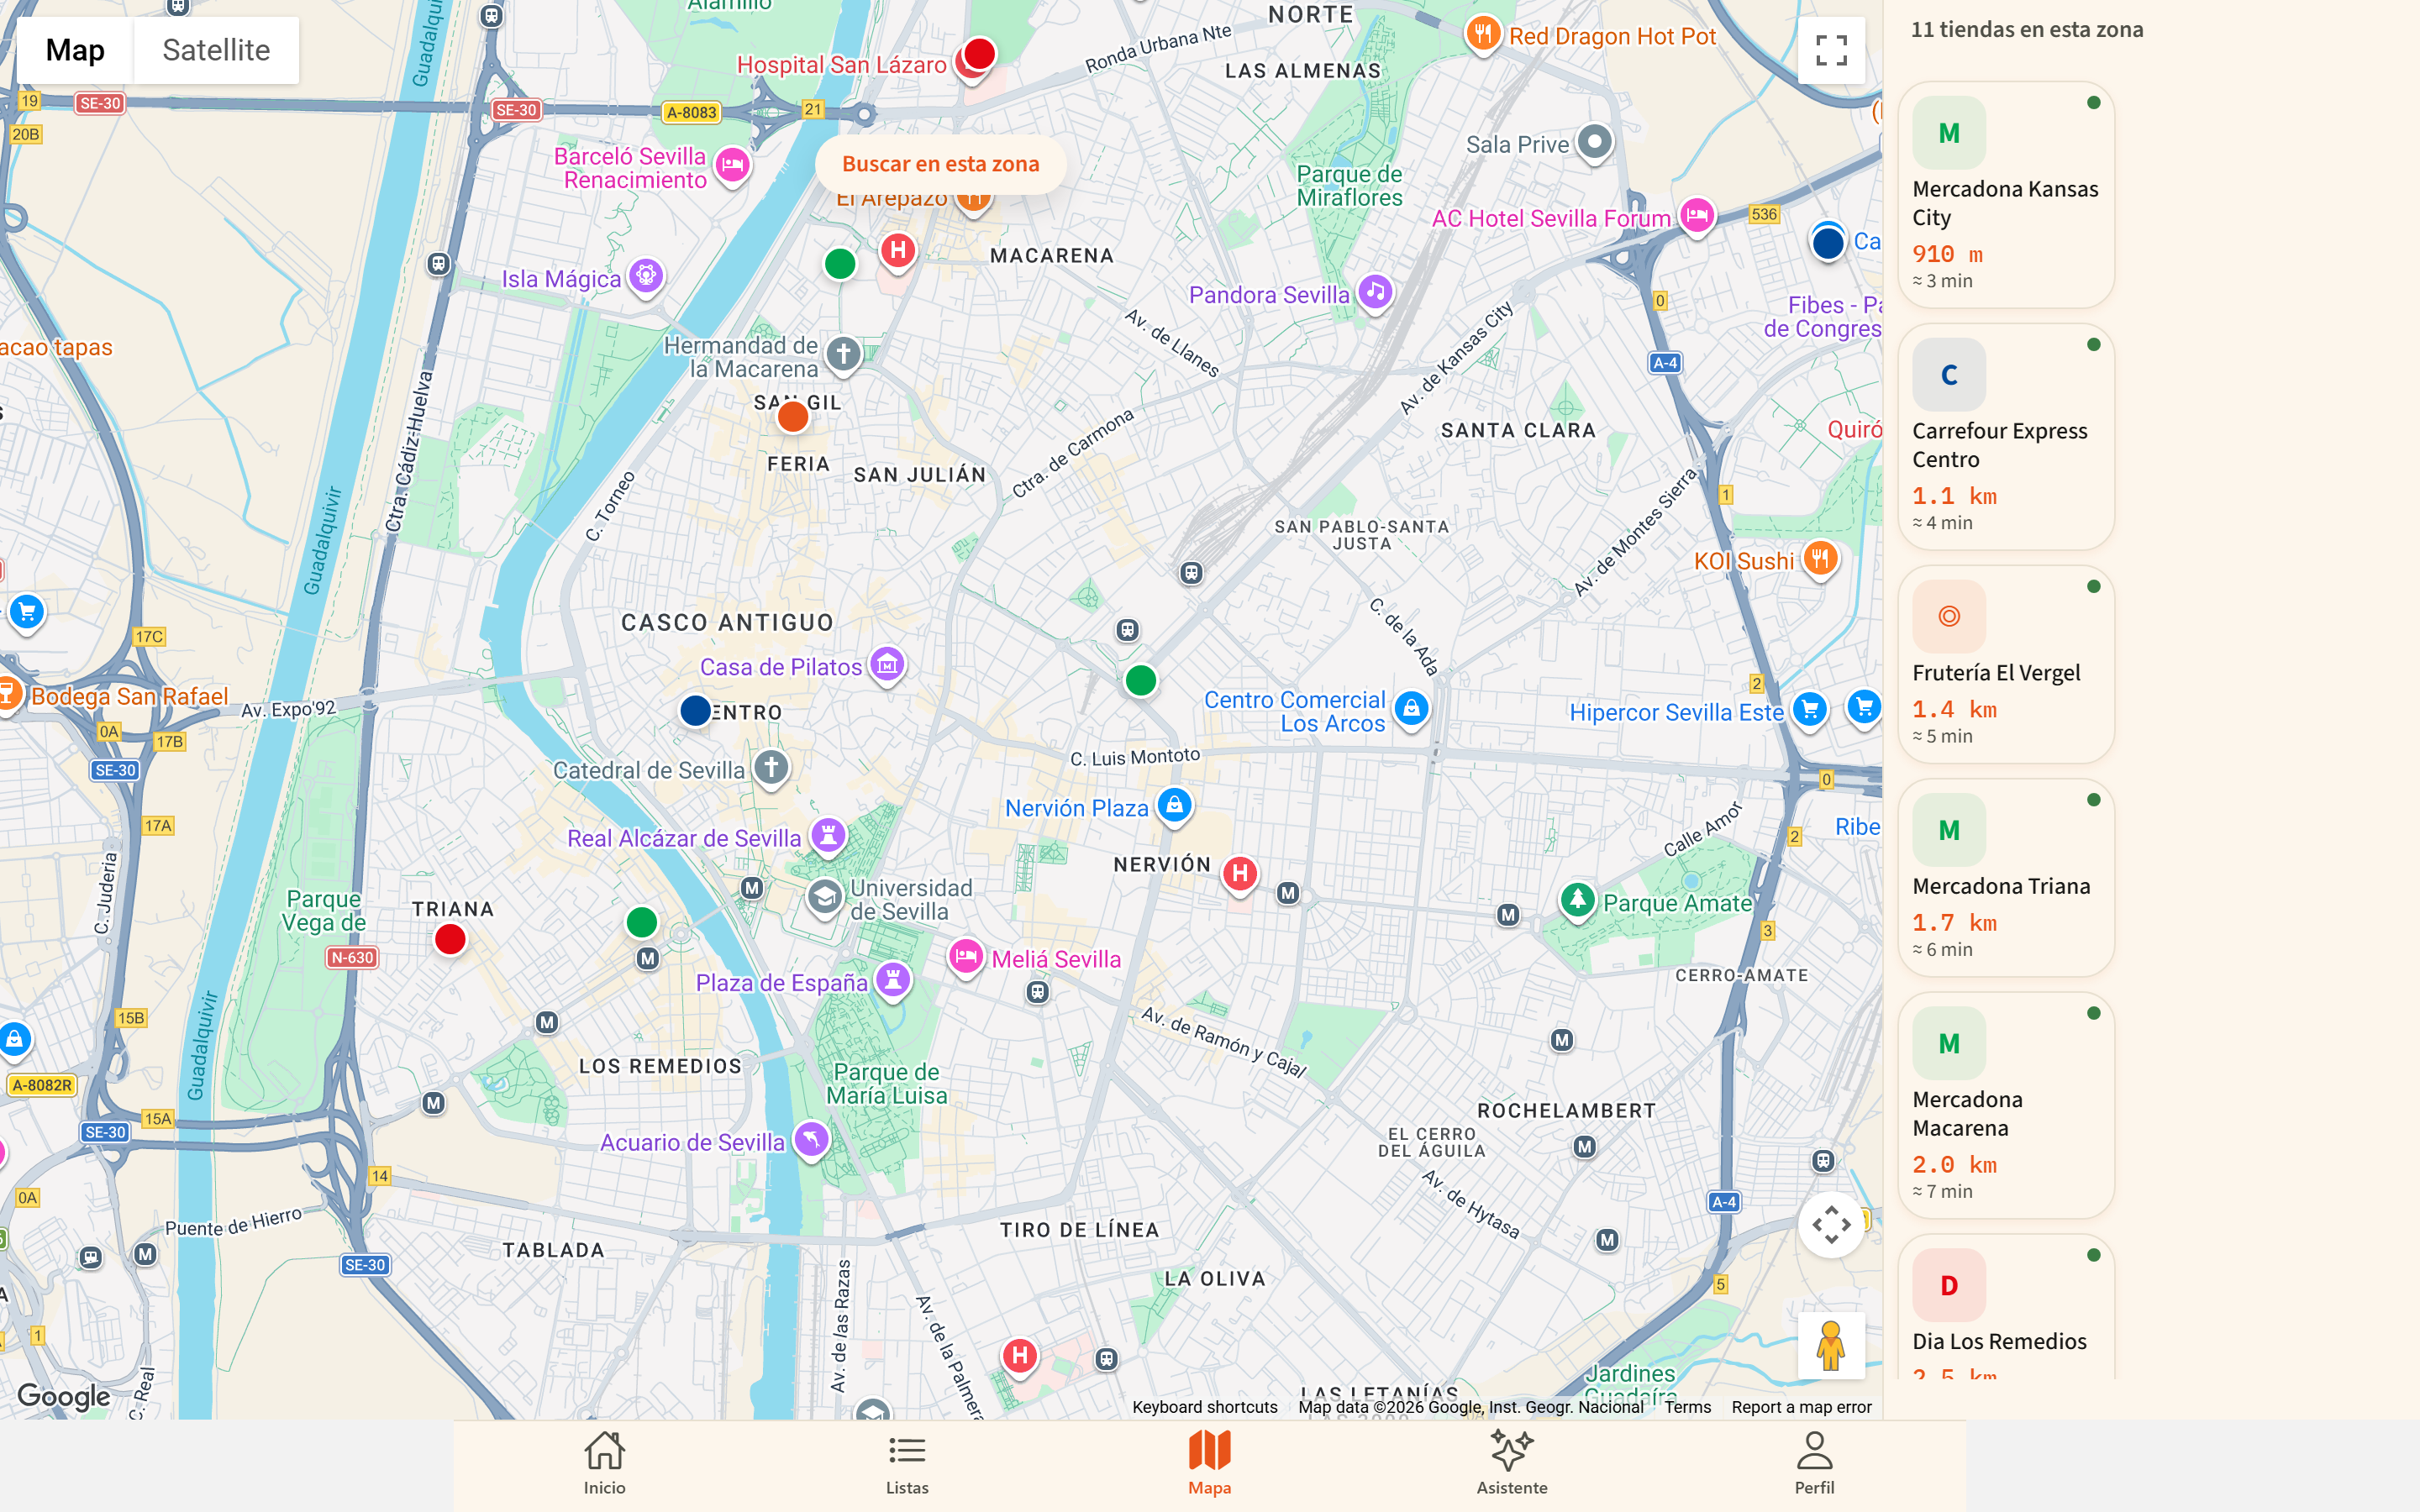
\includegraphics[width=0.48\textwidth]{diagramas/capturas/web-mapa.png}
\hfill
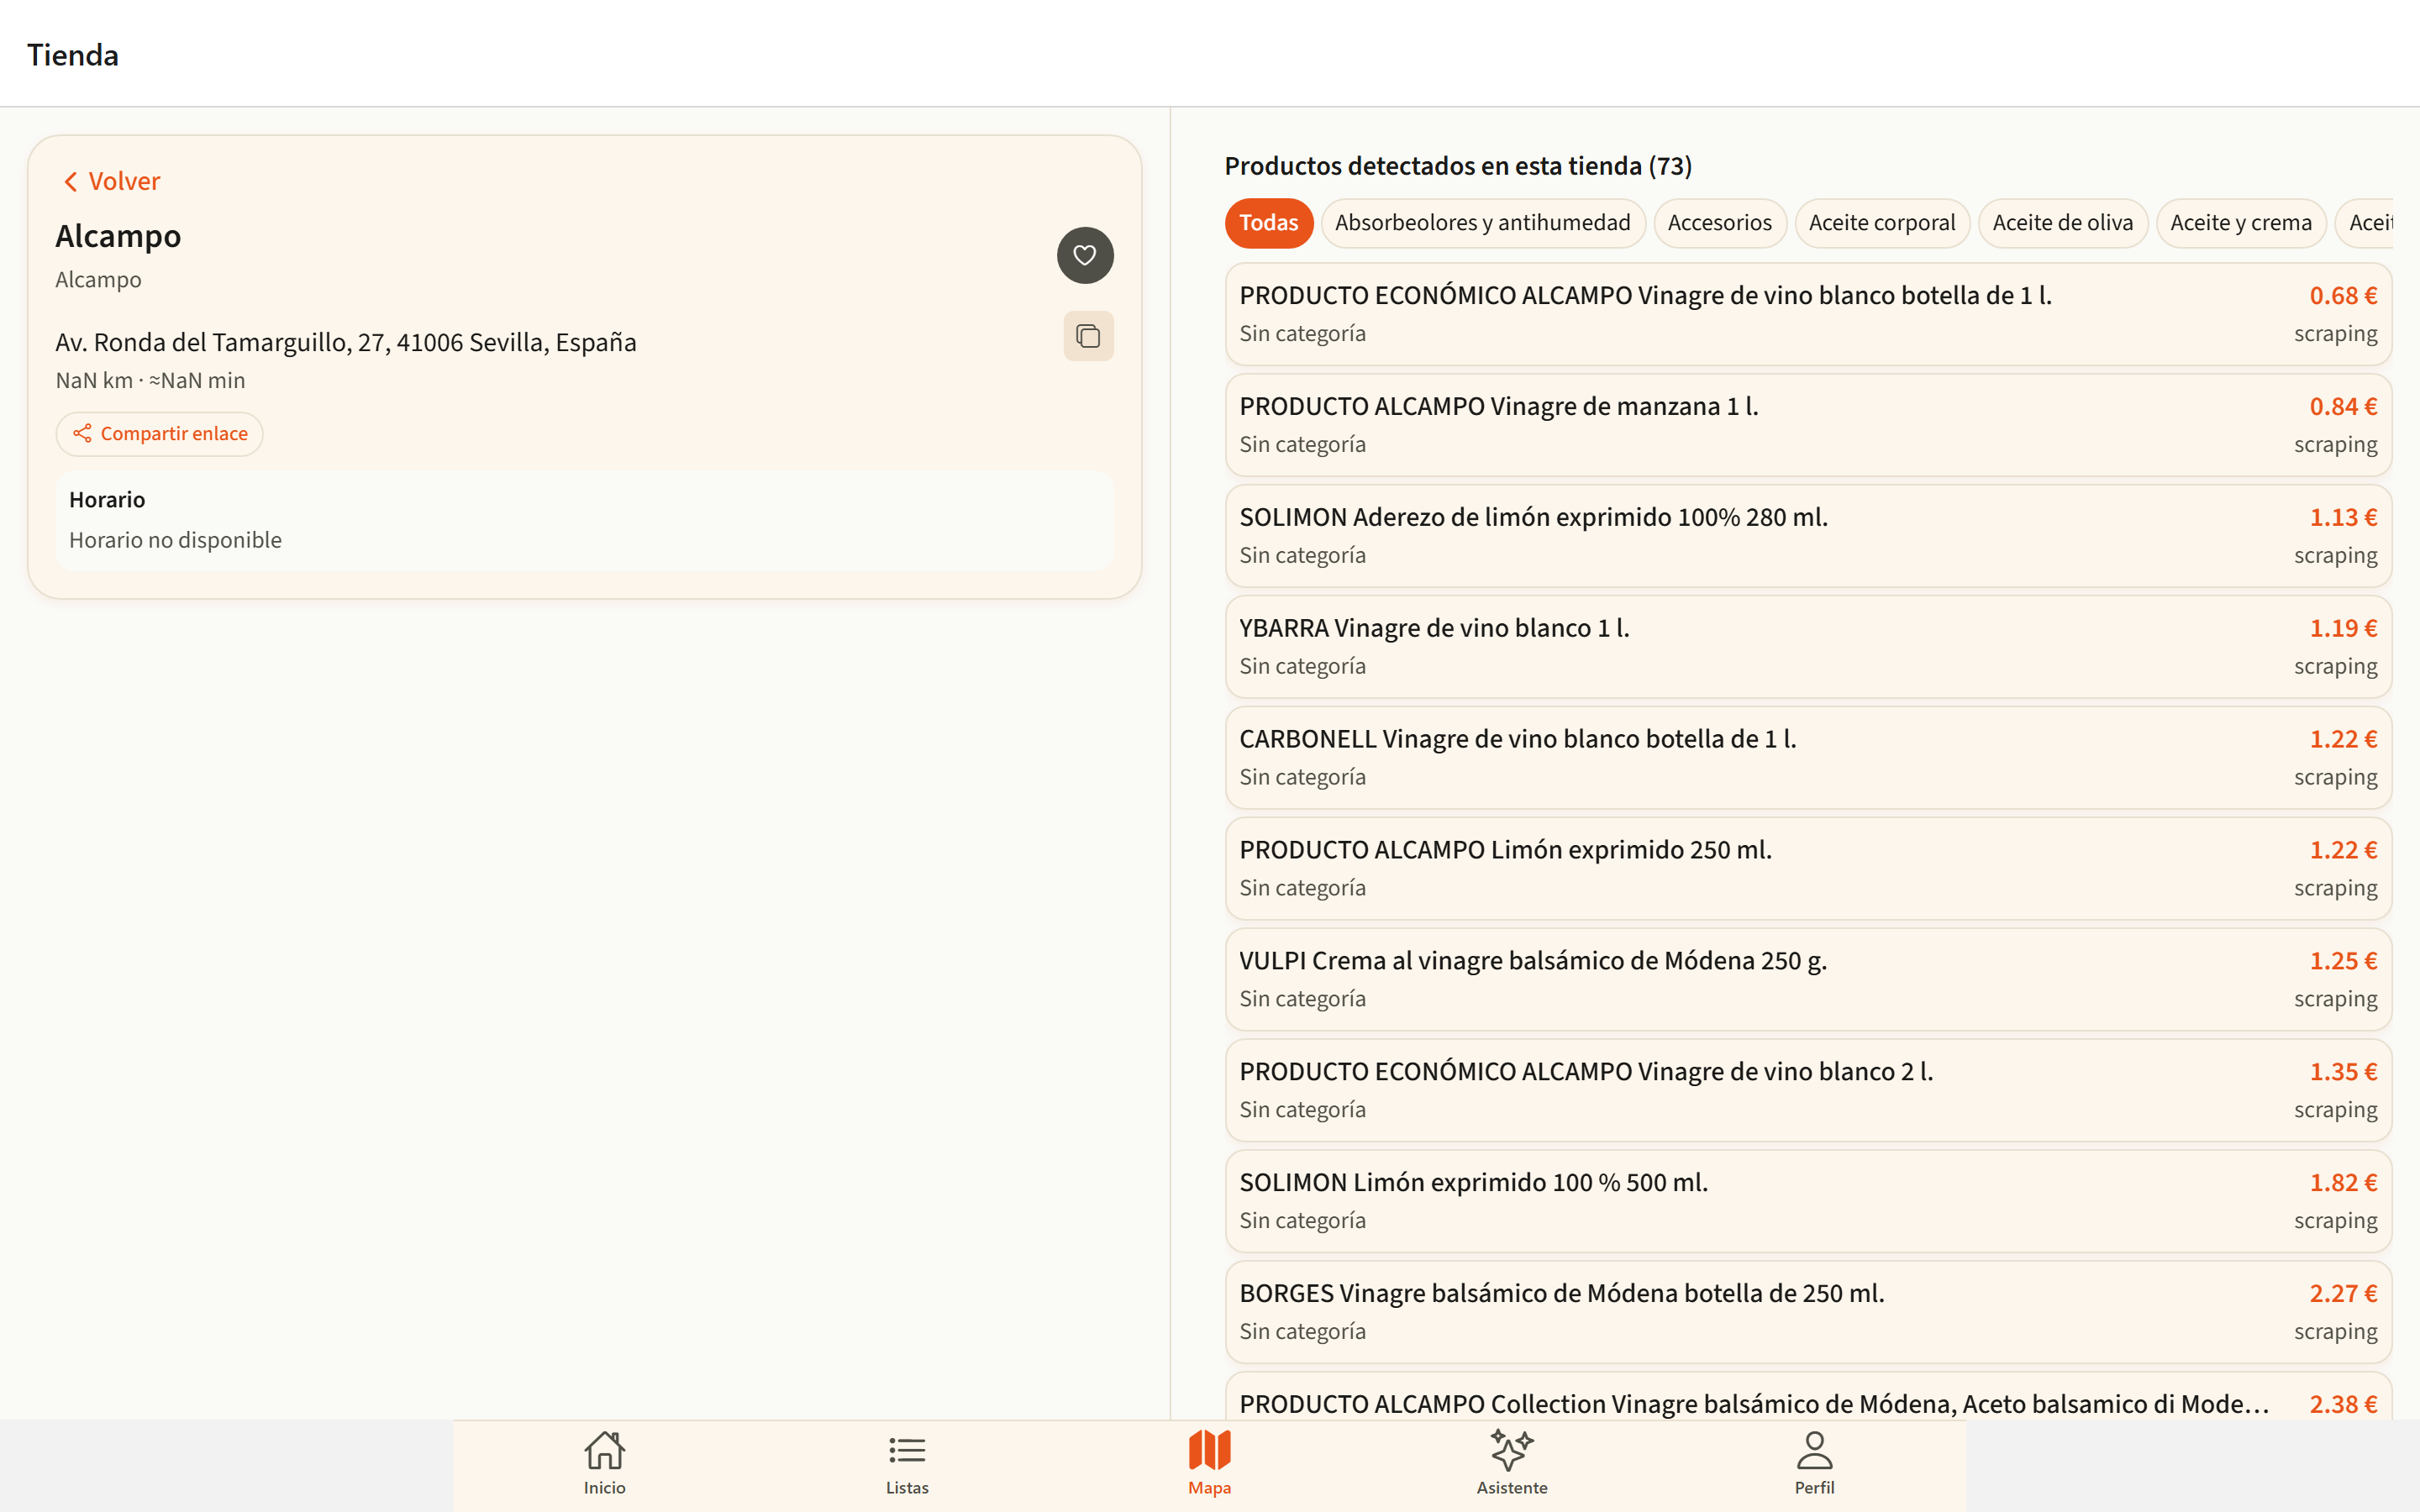
\includegraphics[width=0.48\textwidth]{diagramas/capturas/web-tienda-perfil.png}
\caption{Mapa con panel lateral de tiendas (izquierda) y perfil de tienda a dos columnas
(derecha)}
\label{fig:manual-web-mapa}
\end{figure}

\begin{figure}[htbp]
\centering
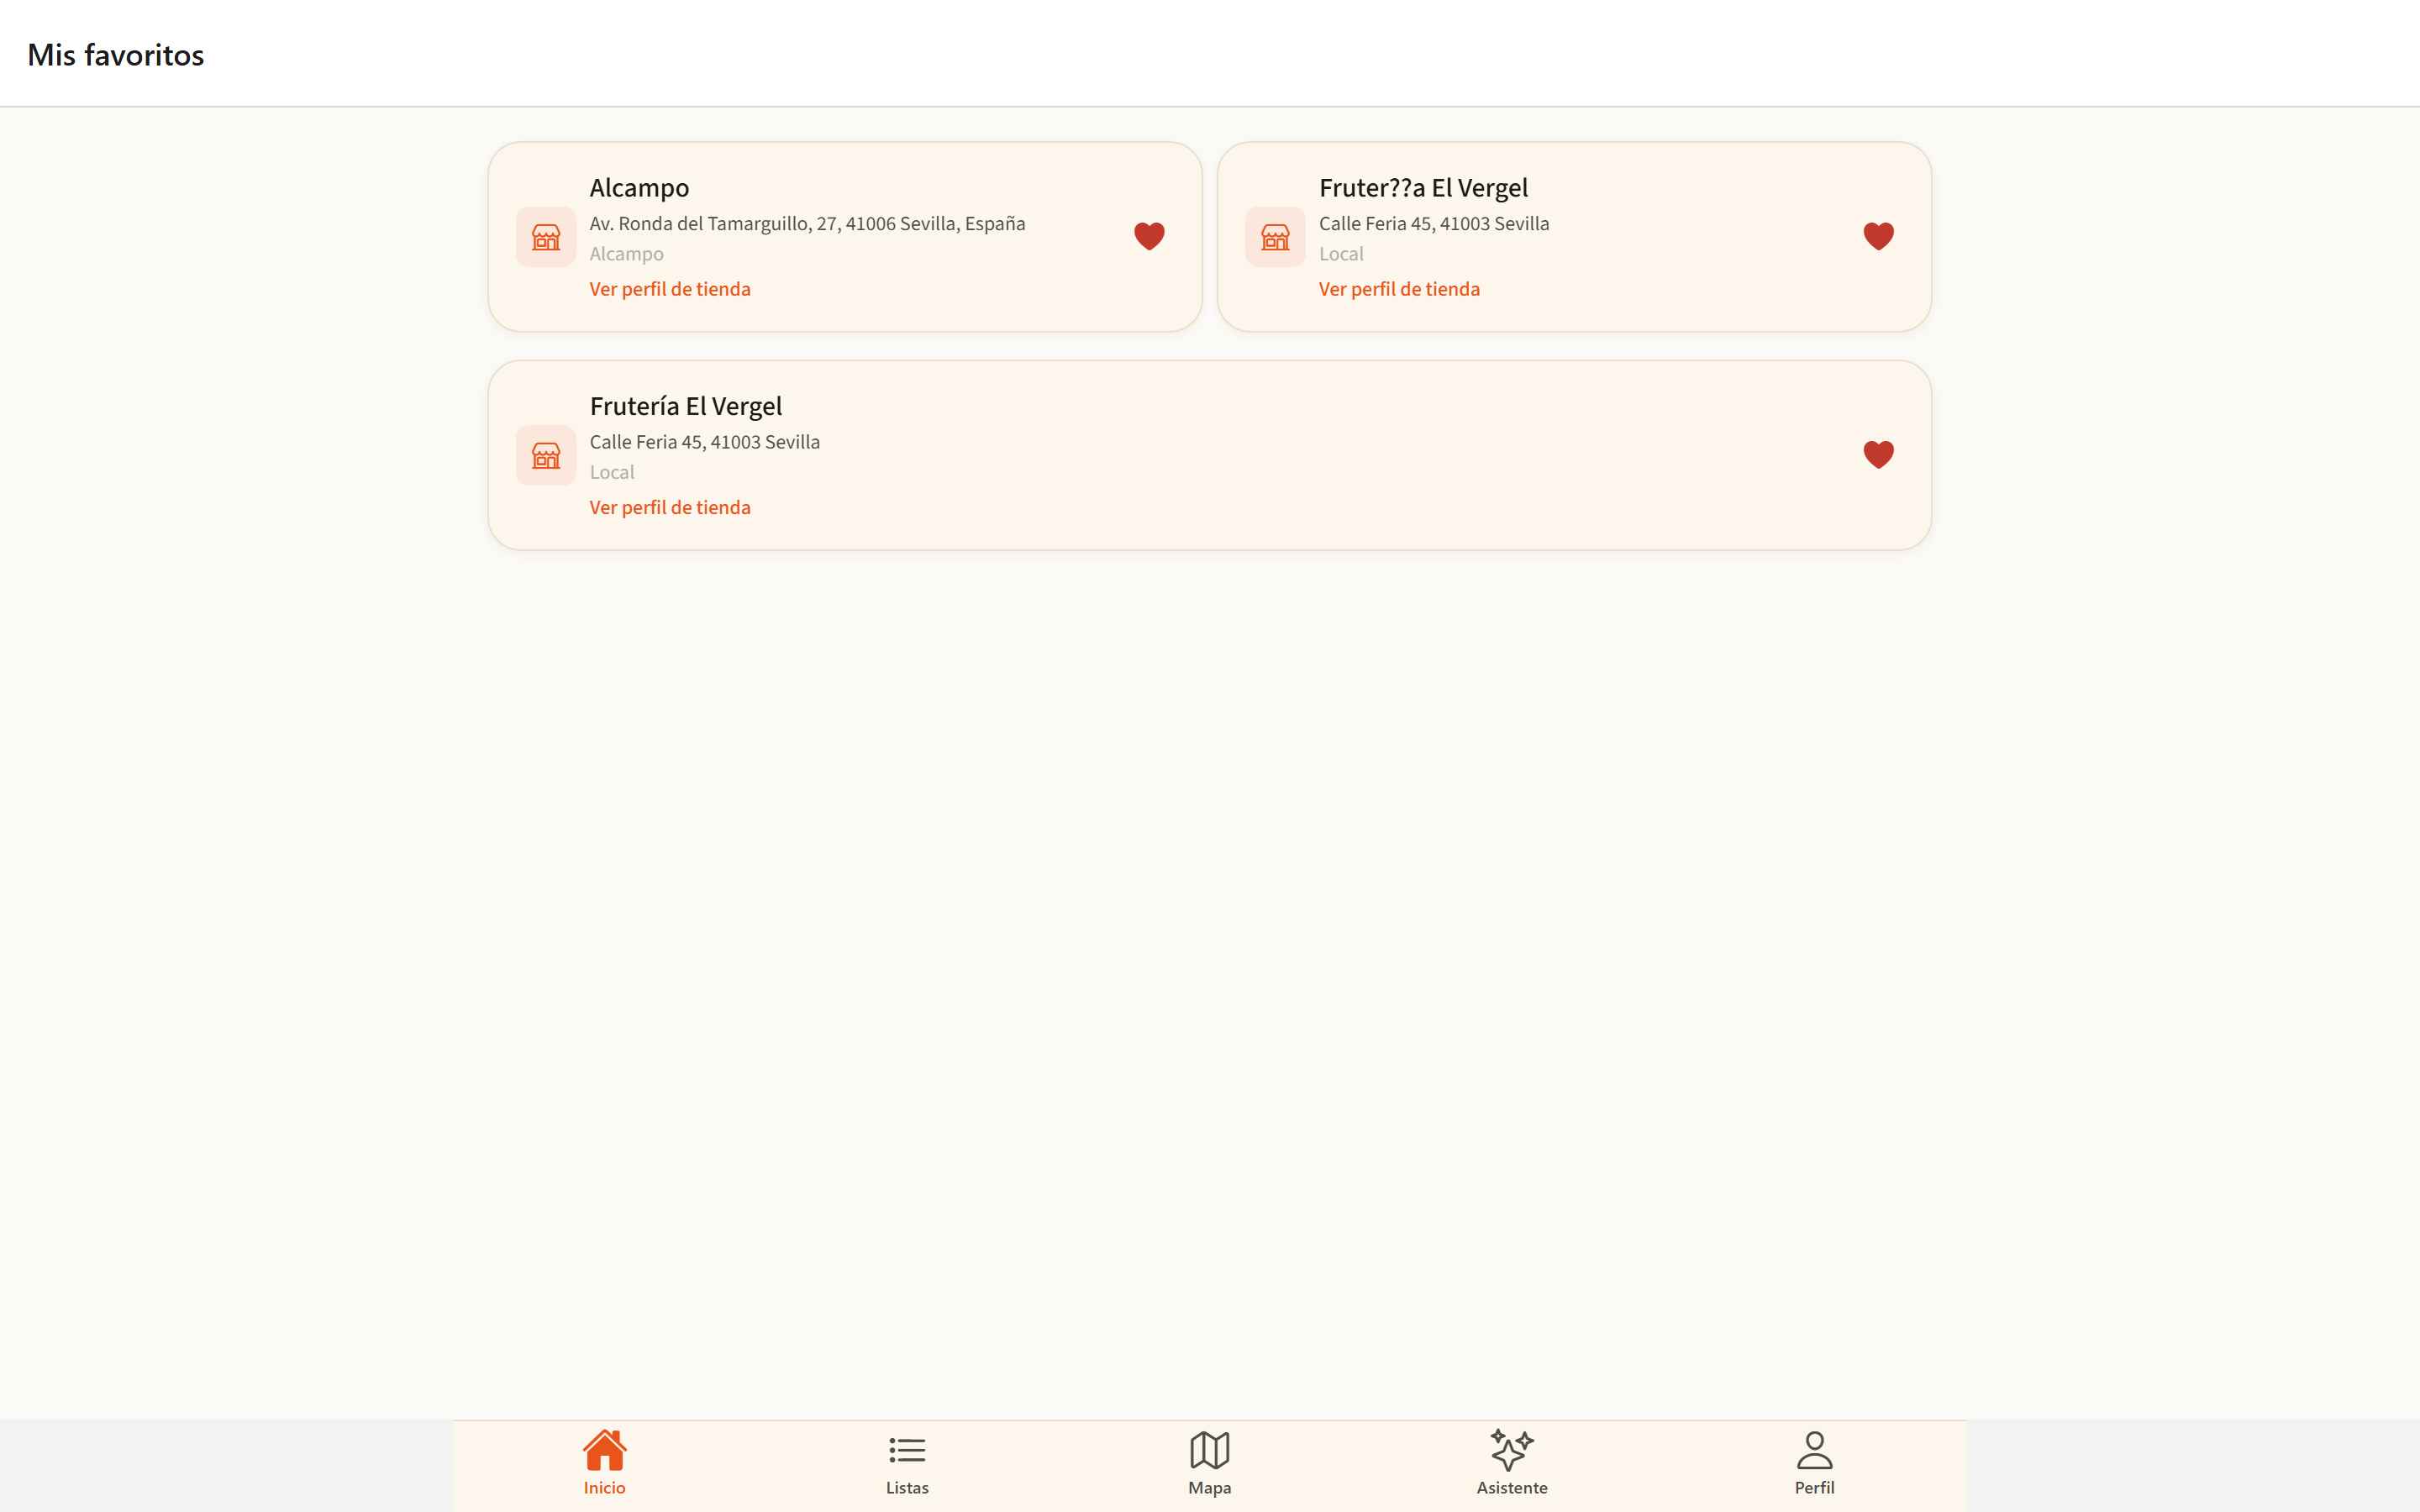
\includegraphics[width=0.48\textwidth]{diagramas/capturas/web-favoritas.png}
\hfill
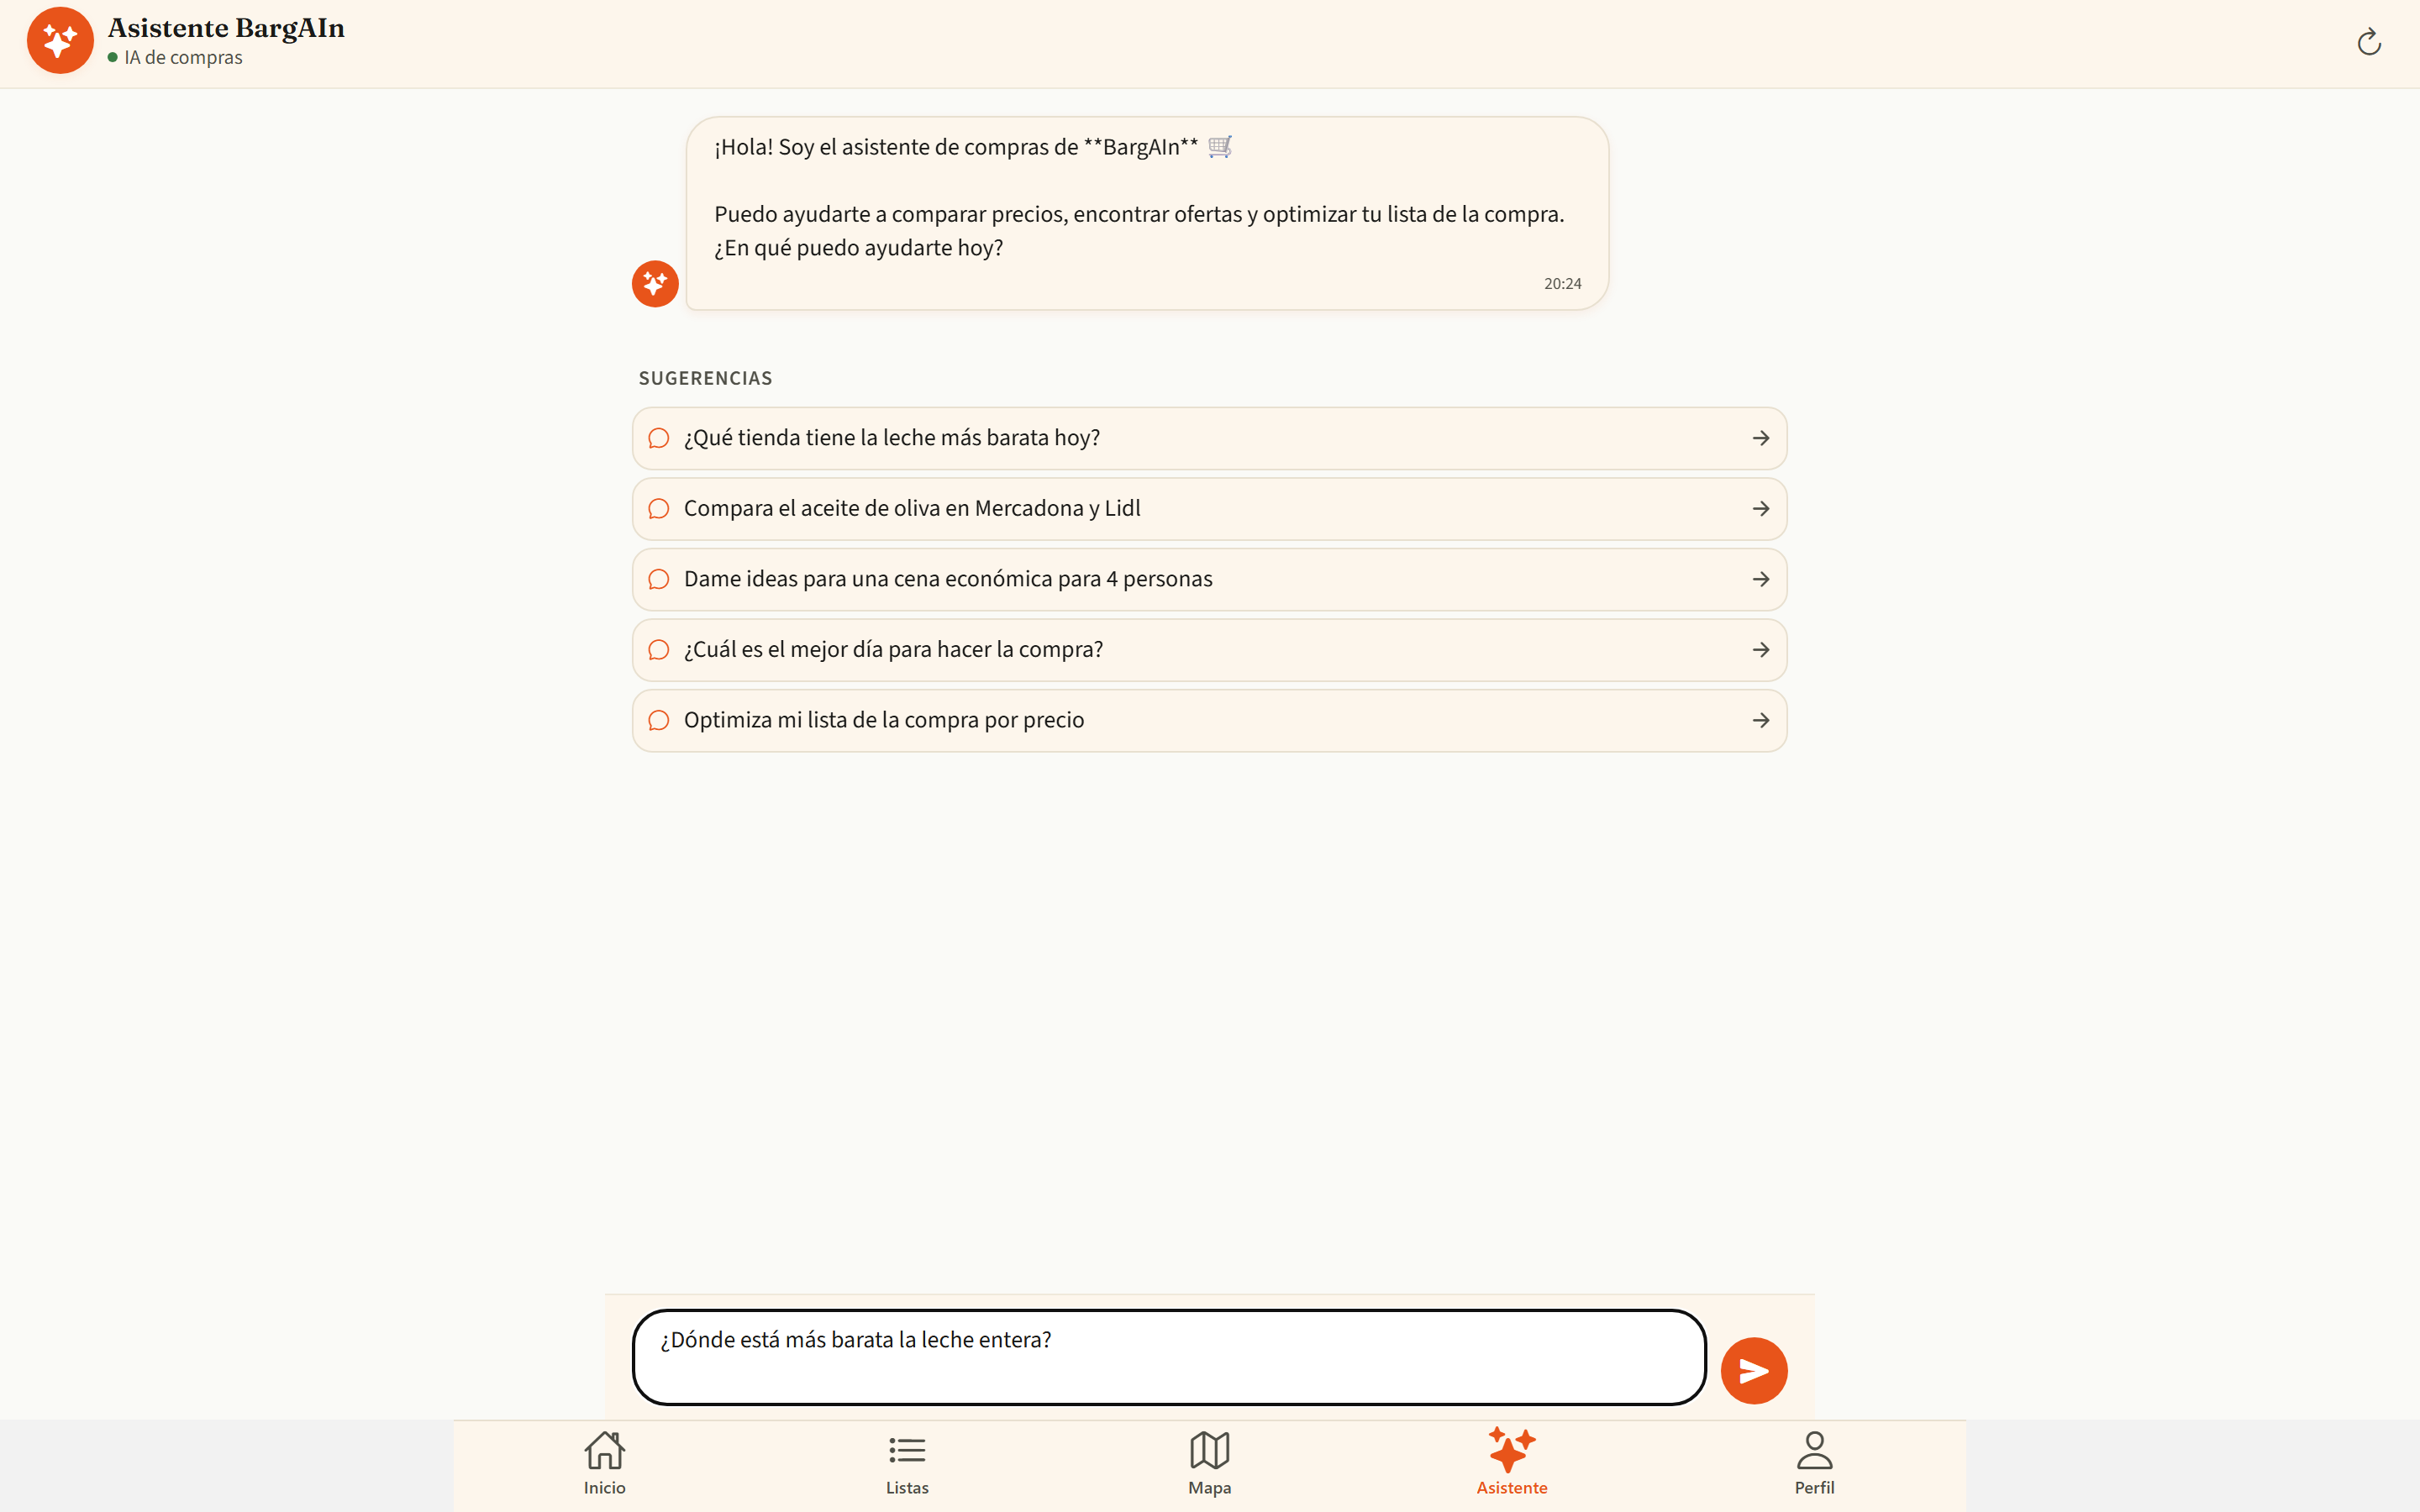
\includegraphics[width=0.48\textwidth]{diagramas/capturas/web-asistente.png}
\caption{Tiendas favoritas en rejilla (izquierda) y asistente conversacional centrado con copia
por mensaje (derecha)}
\label{fig:manual-web-favoritas}
\end{figure}

\begin{figure}[htbp]
\centering
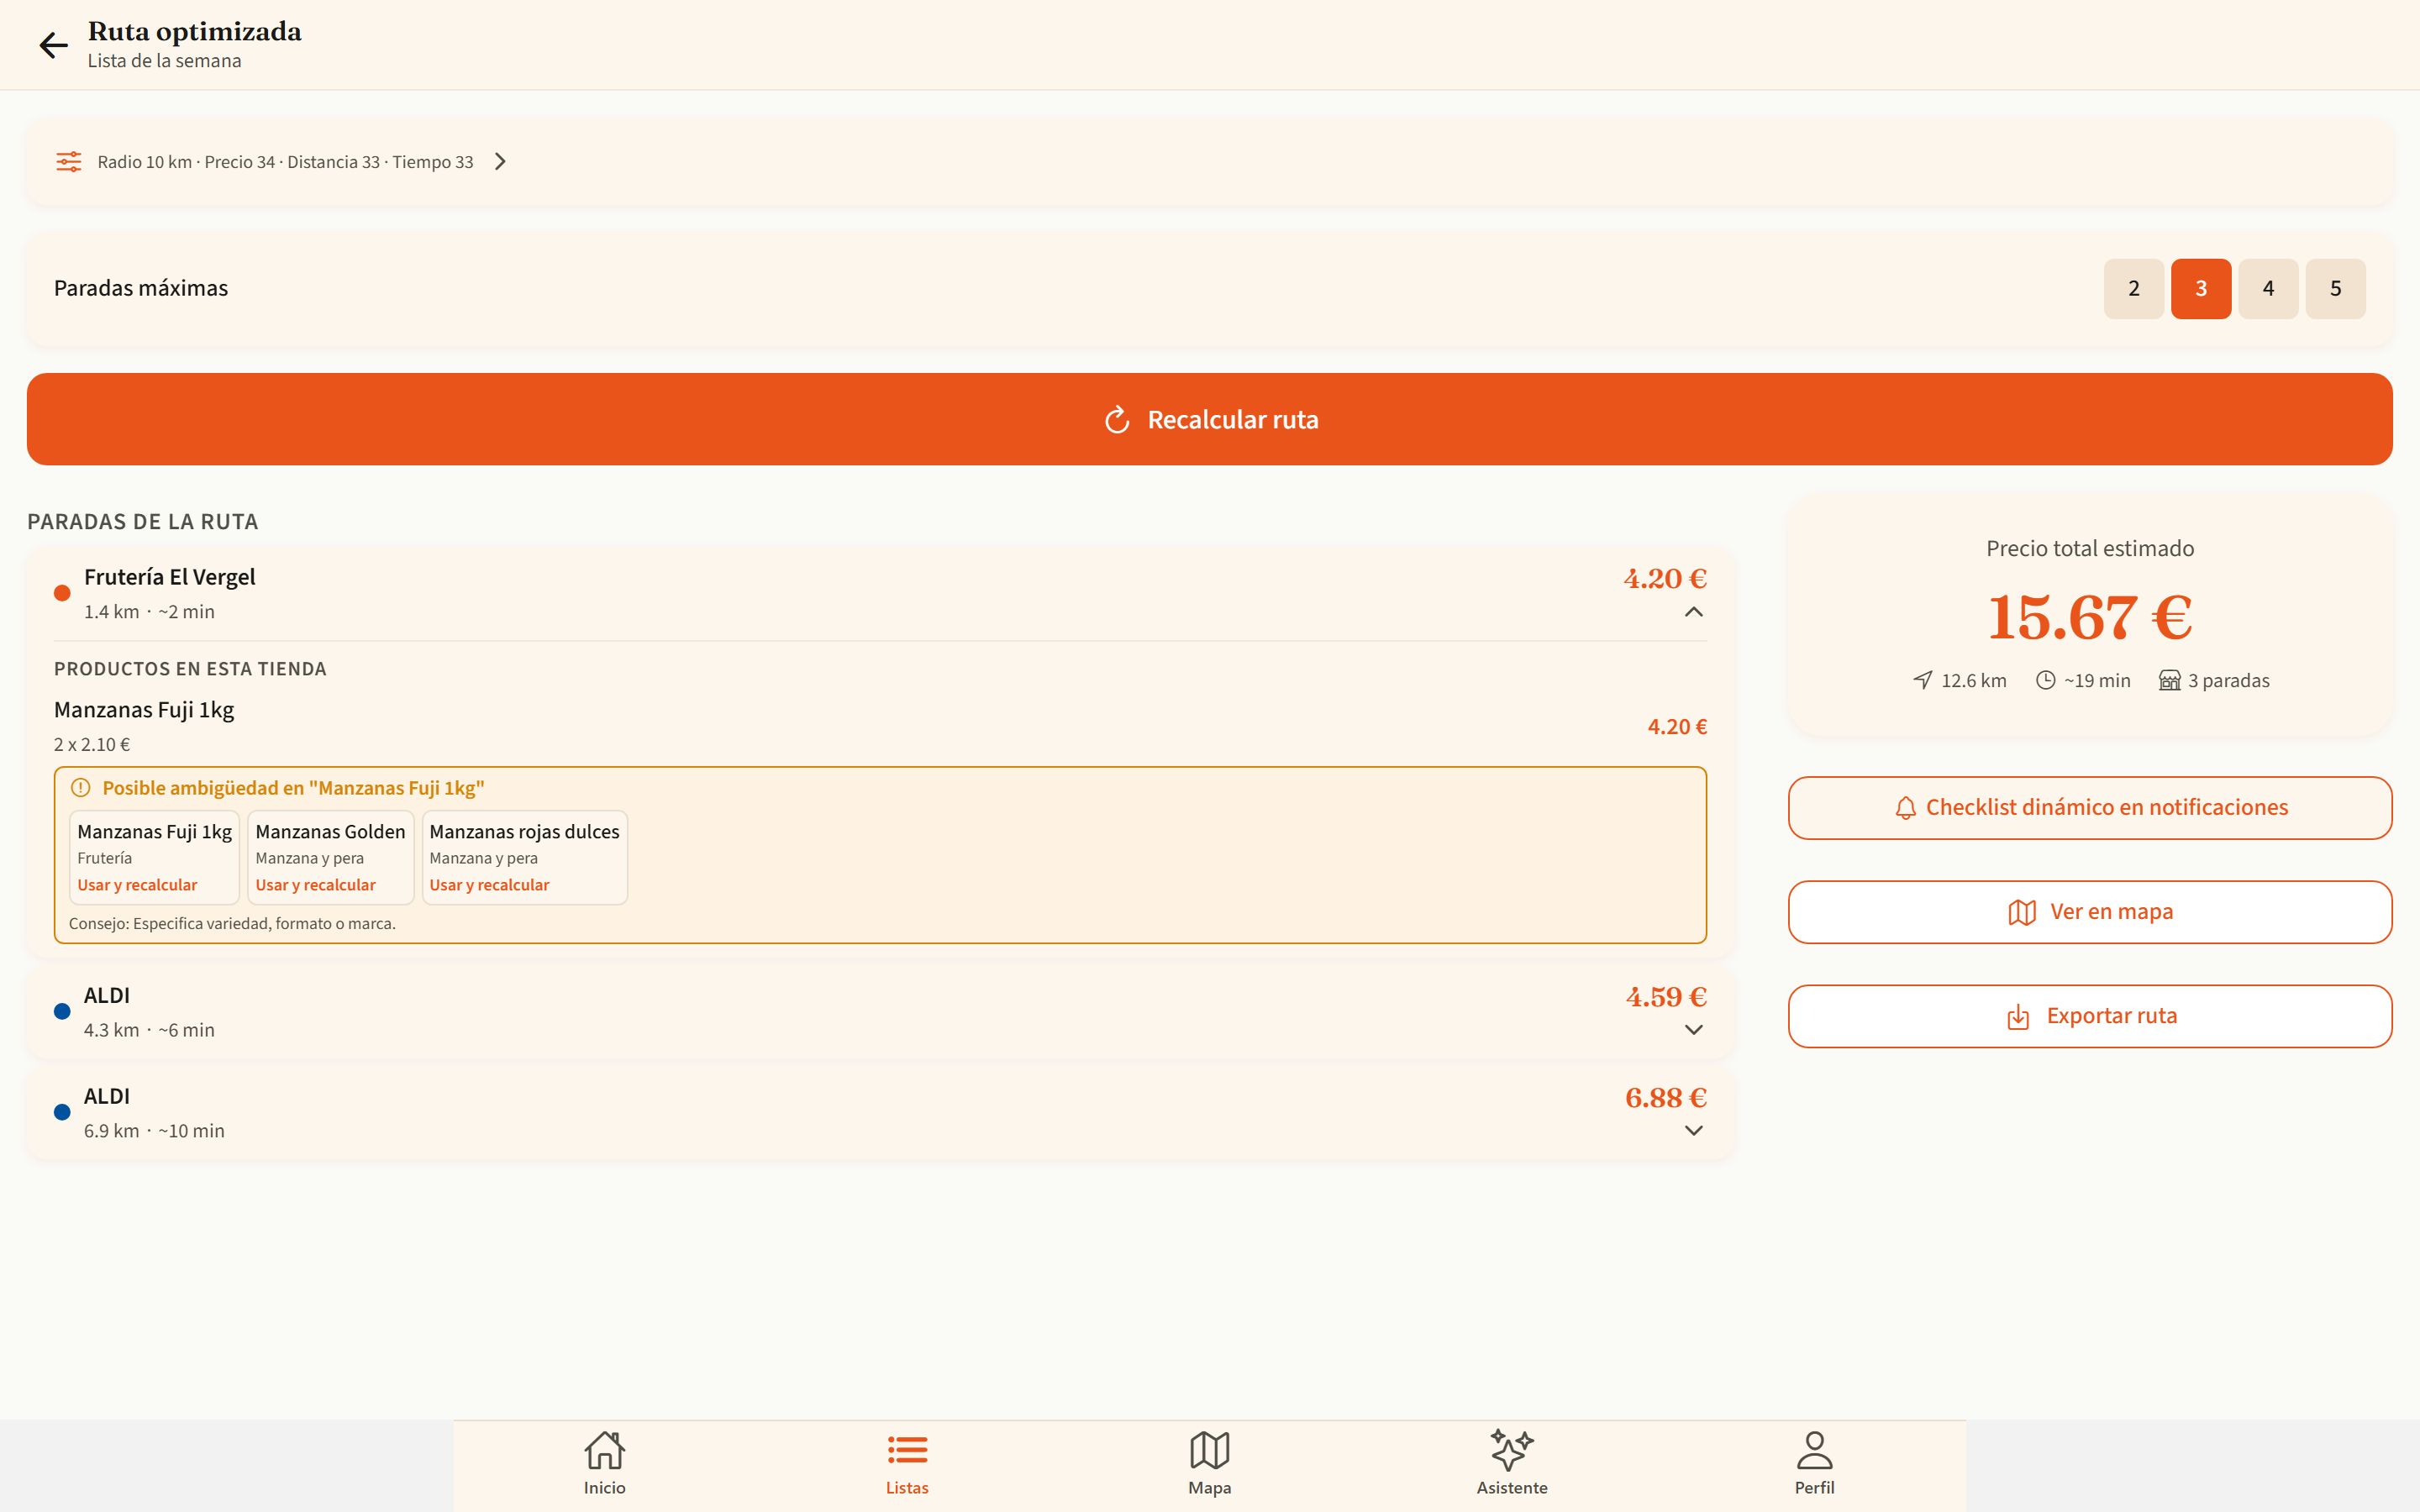
\includegraphics[width=0.48\textwidth]{diagramas/capturas/web-ruta.png}
\hfill
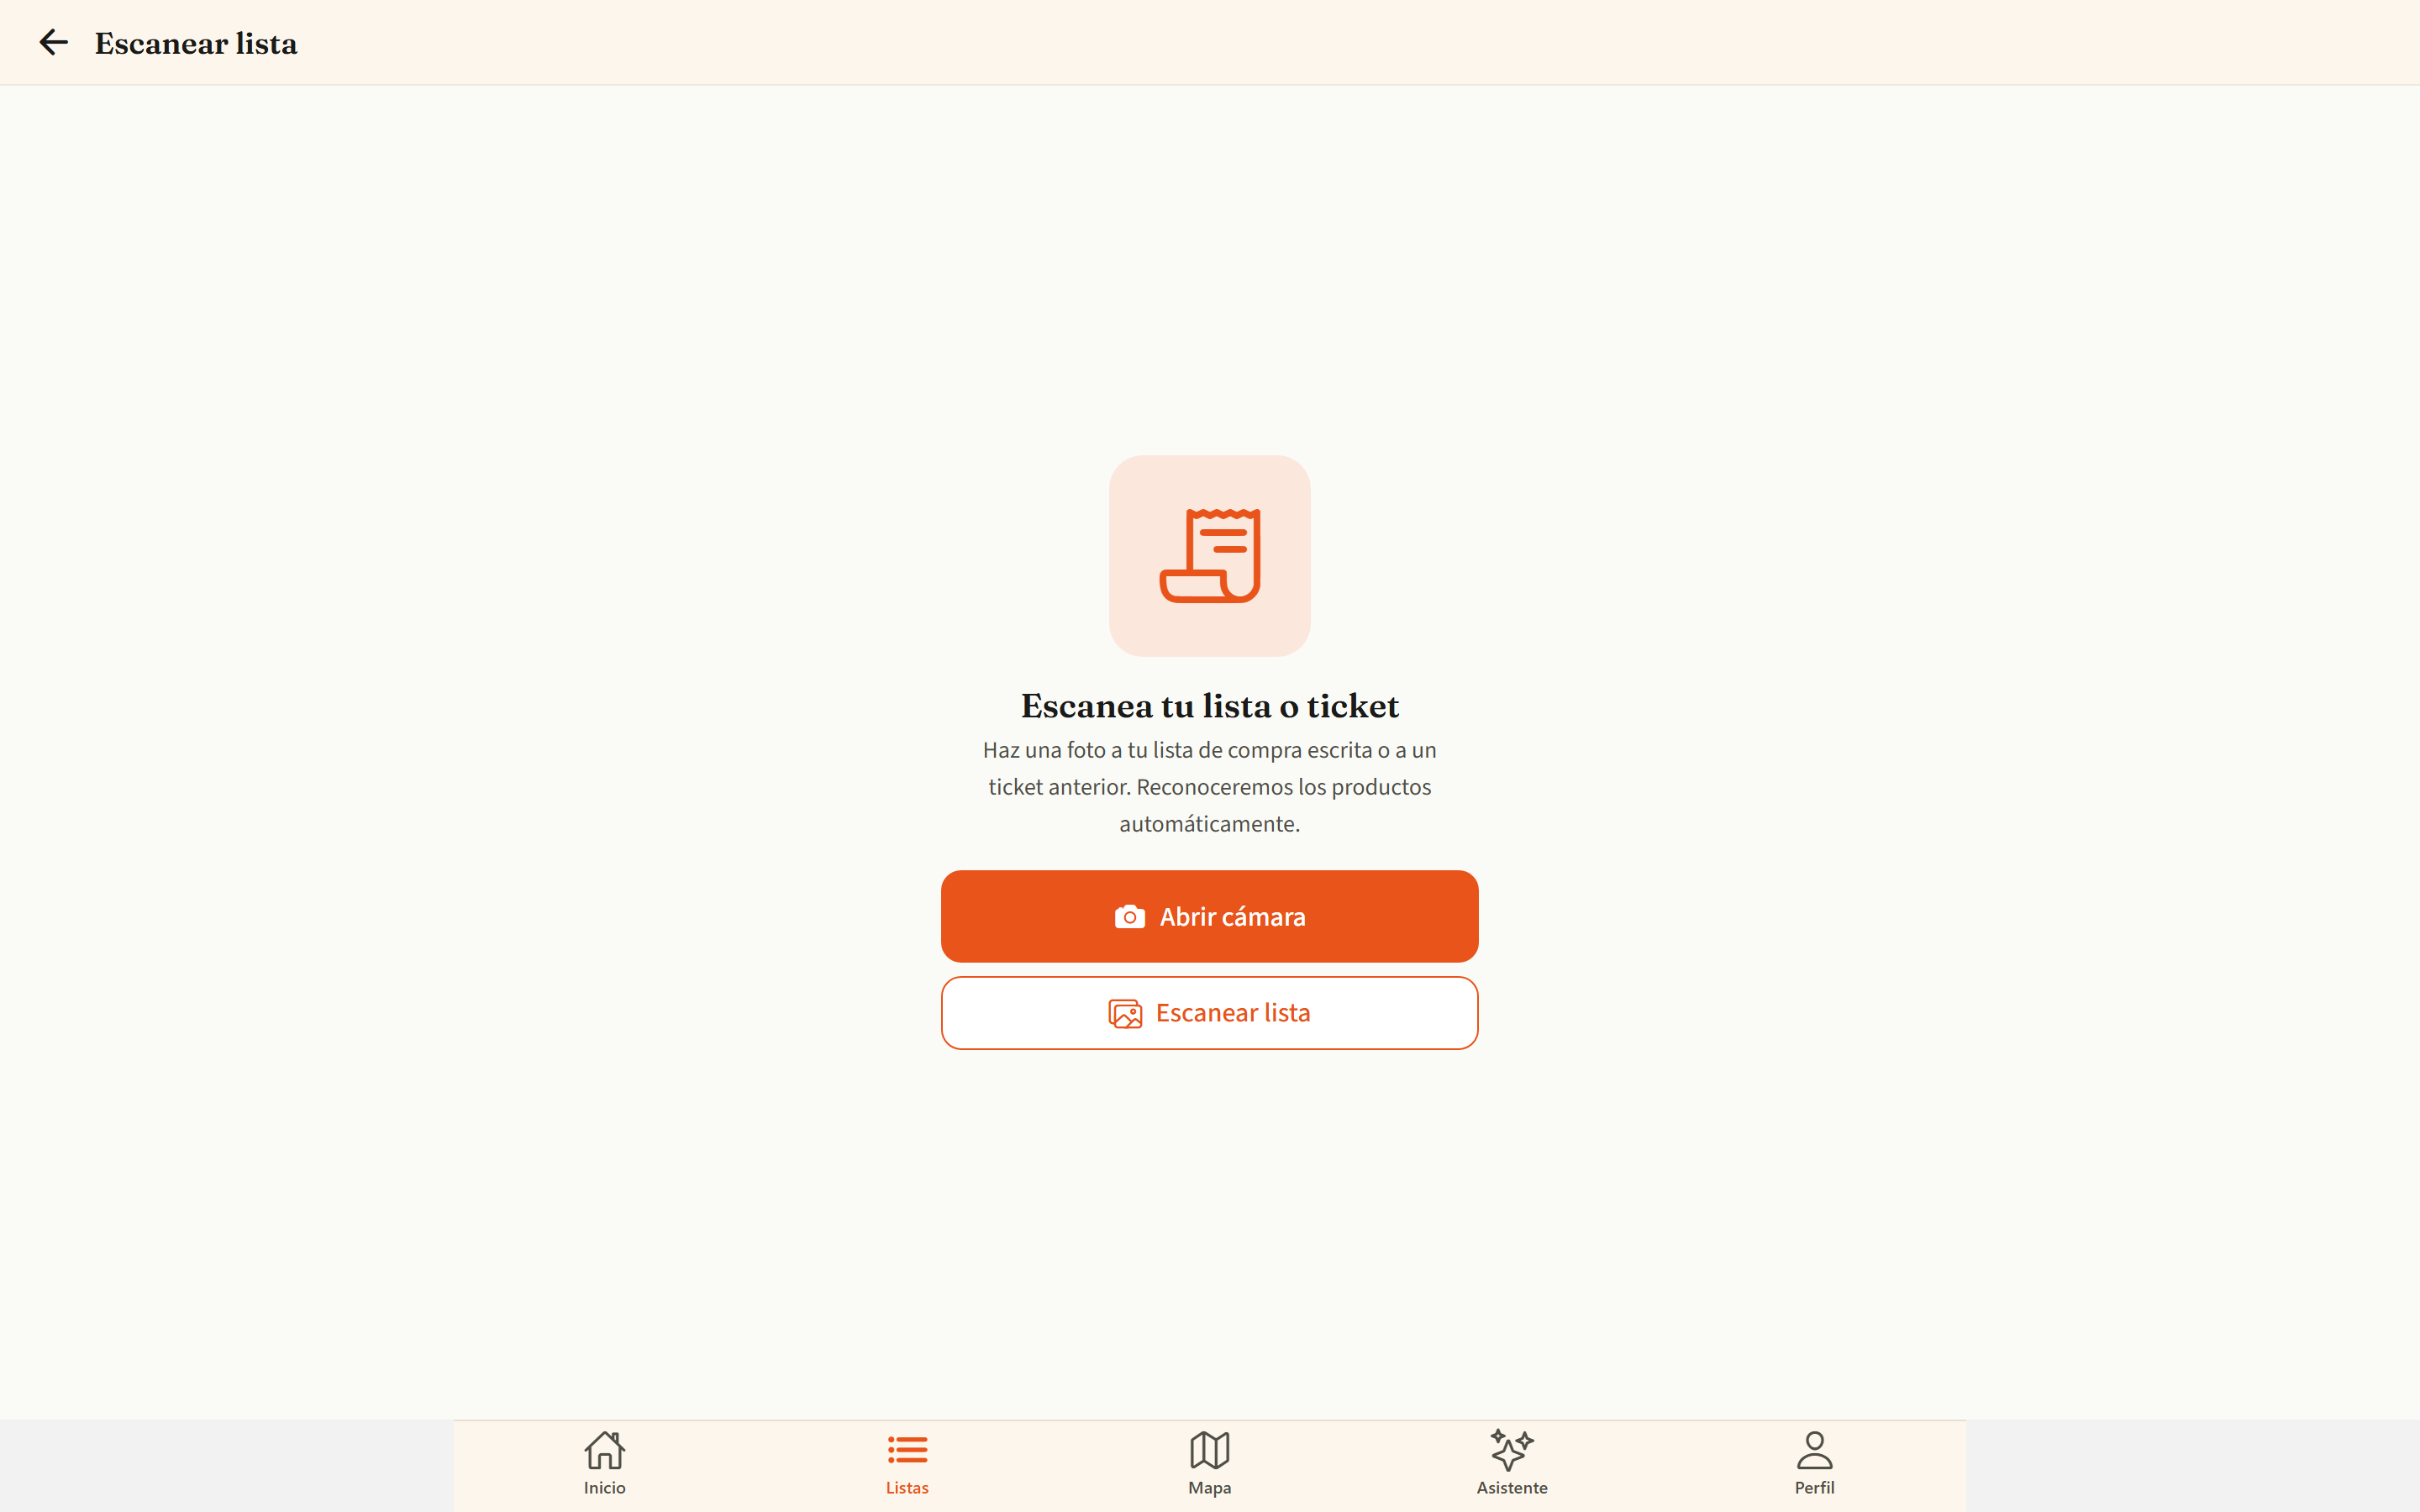
\includegraphics[width=0.48\textwidth]{diagramas/capturas/web-ocr.png}
\caption{Ruta optimizada con exportación del itinerario (izquierda) y módulo OCR adaptado al
escritorio (derecha)}
\label{fig:manual-web-ruta}
\end{figure}

\begin{figure}[htbp]
\centering
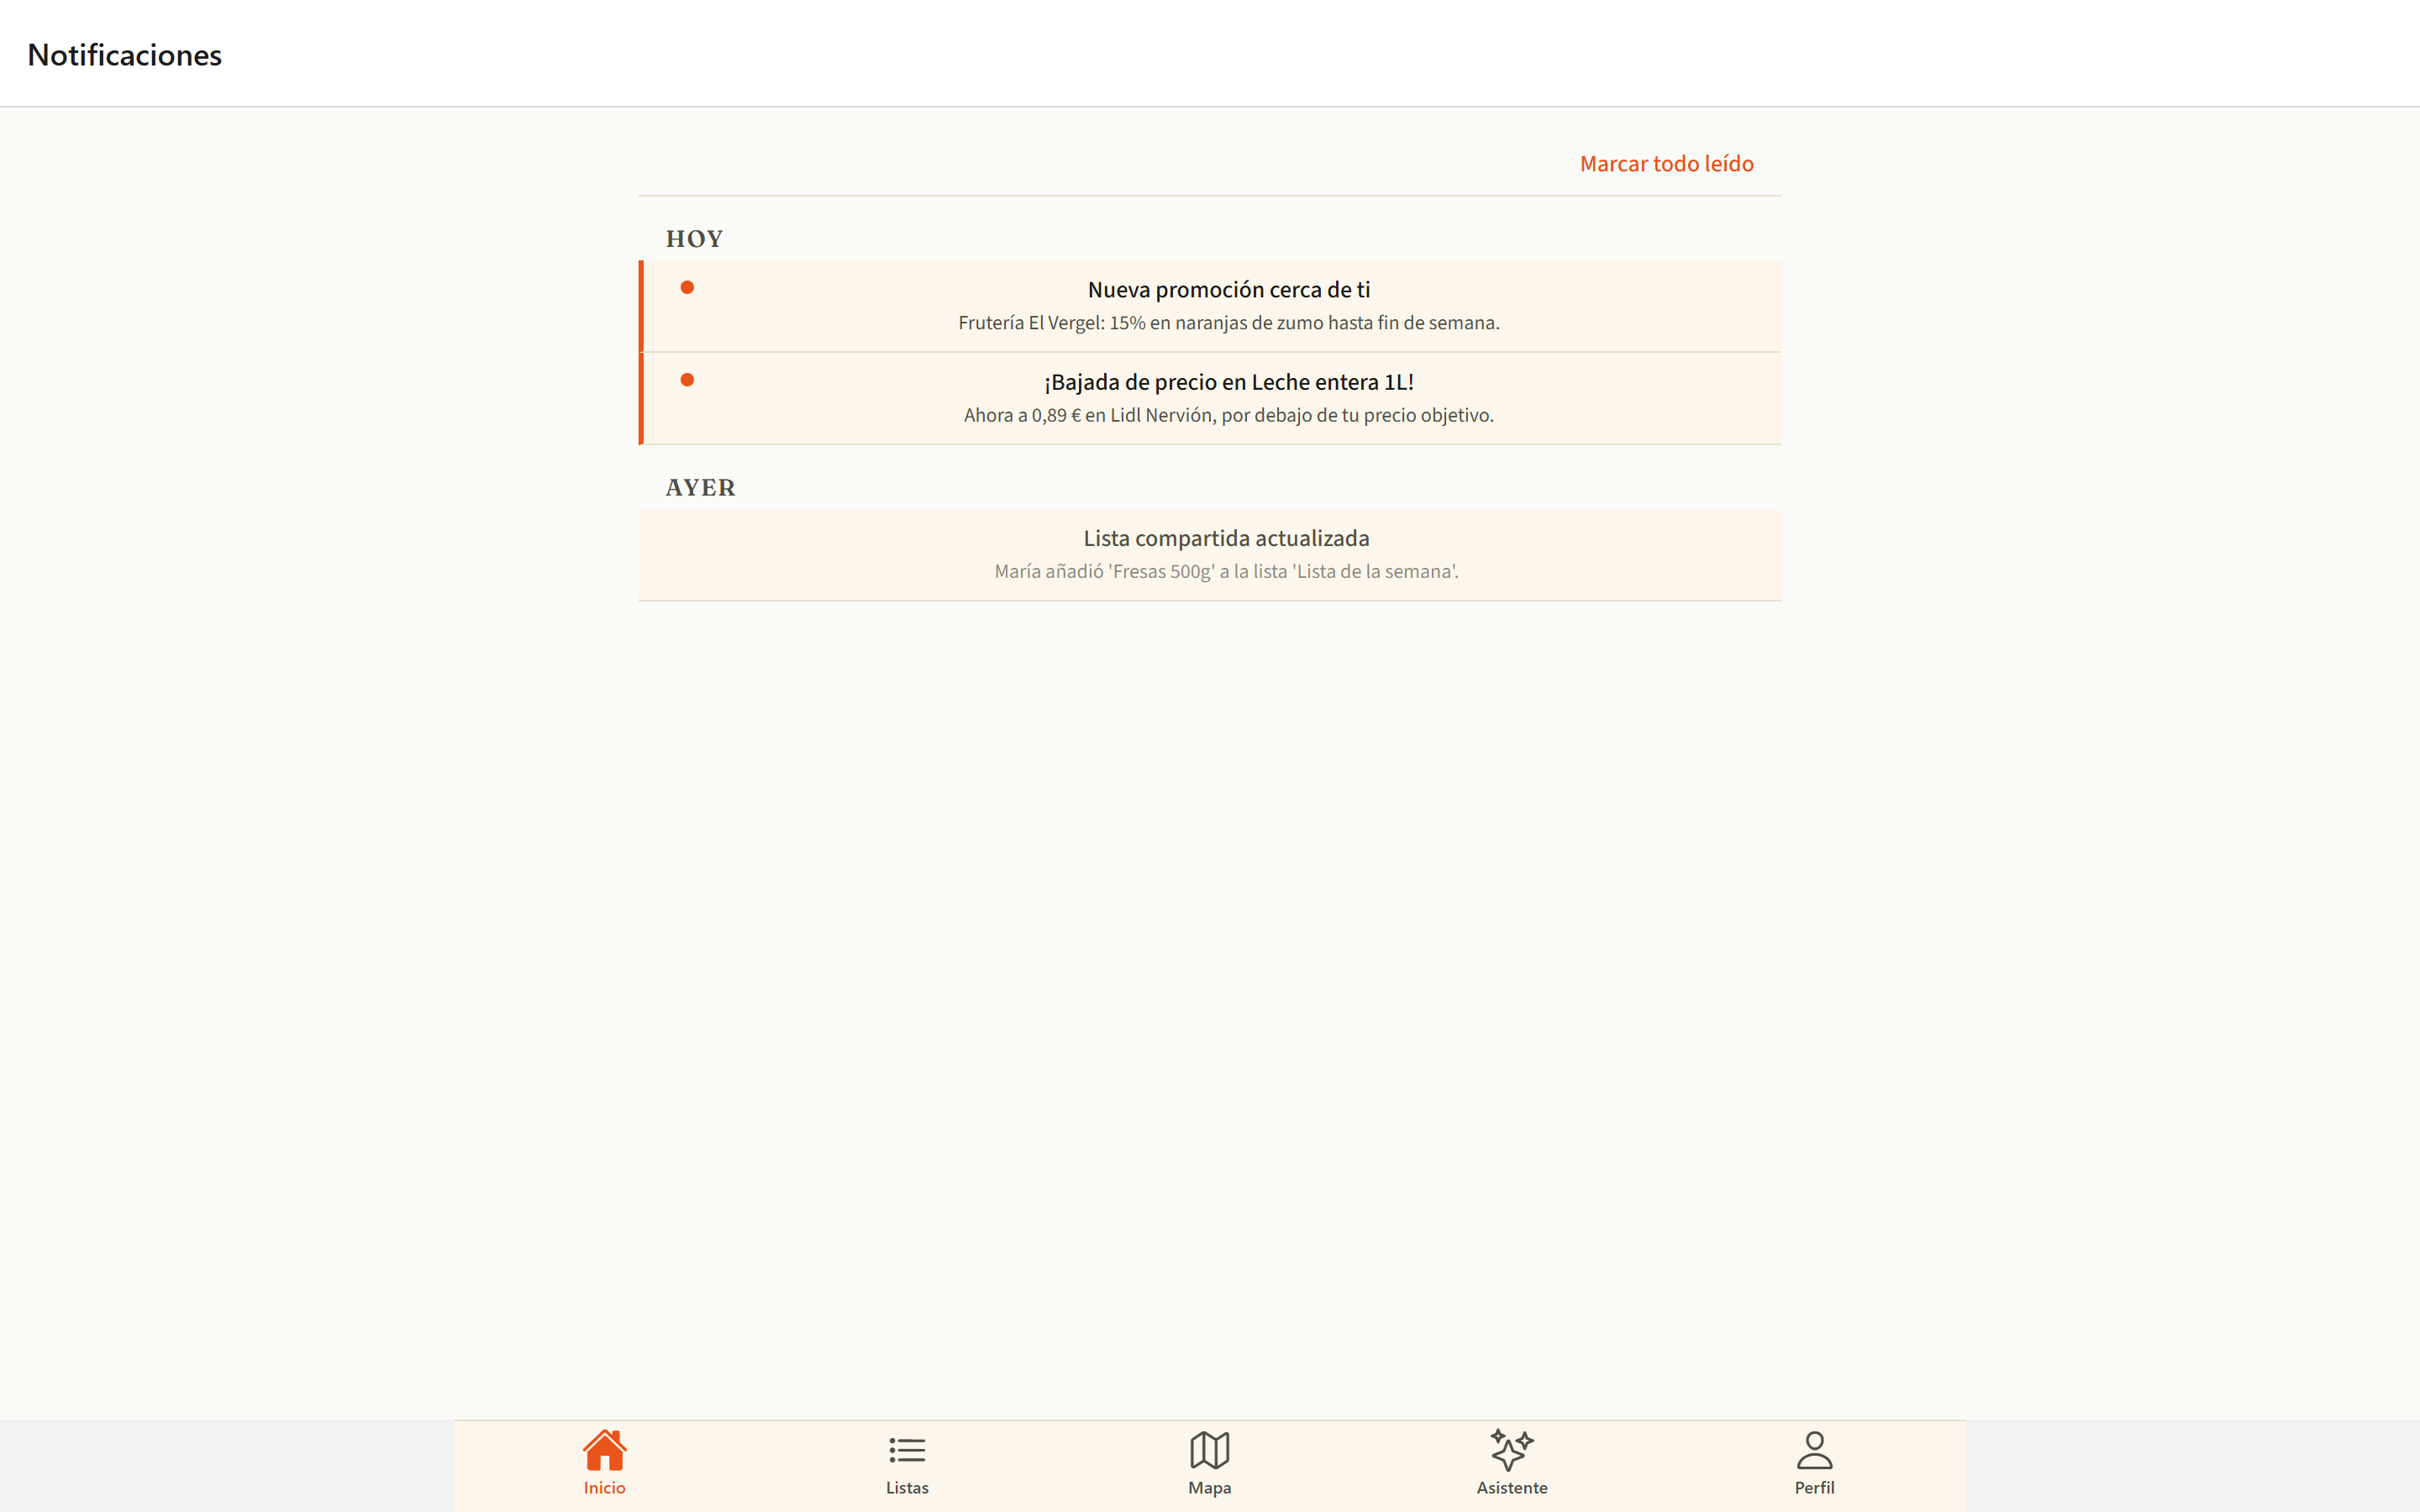
\includegraphics[width=0.48\textwidth]{diagramas/capturas/web-notificaciones.png}
\hfill
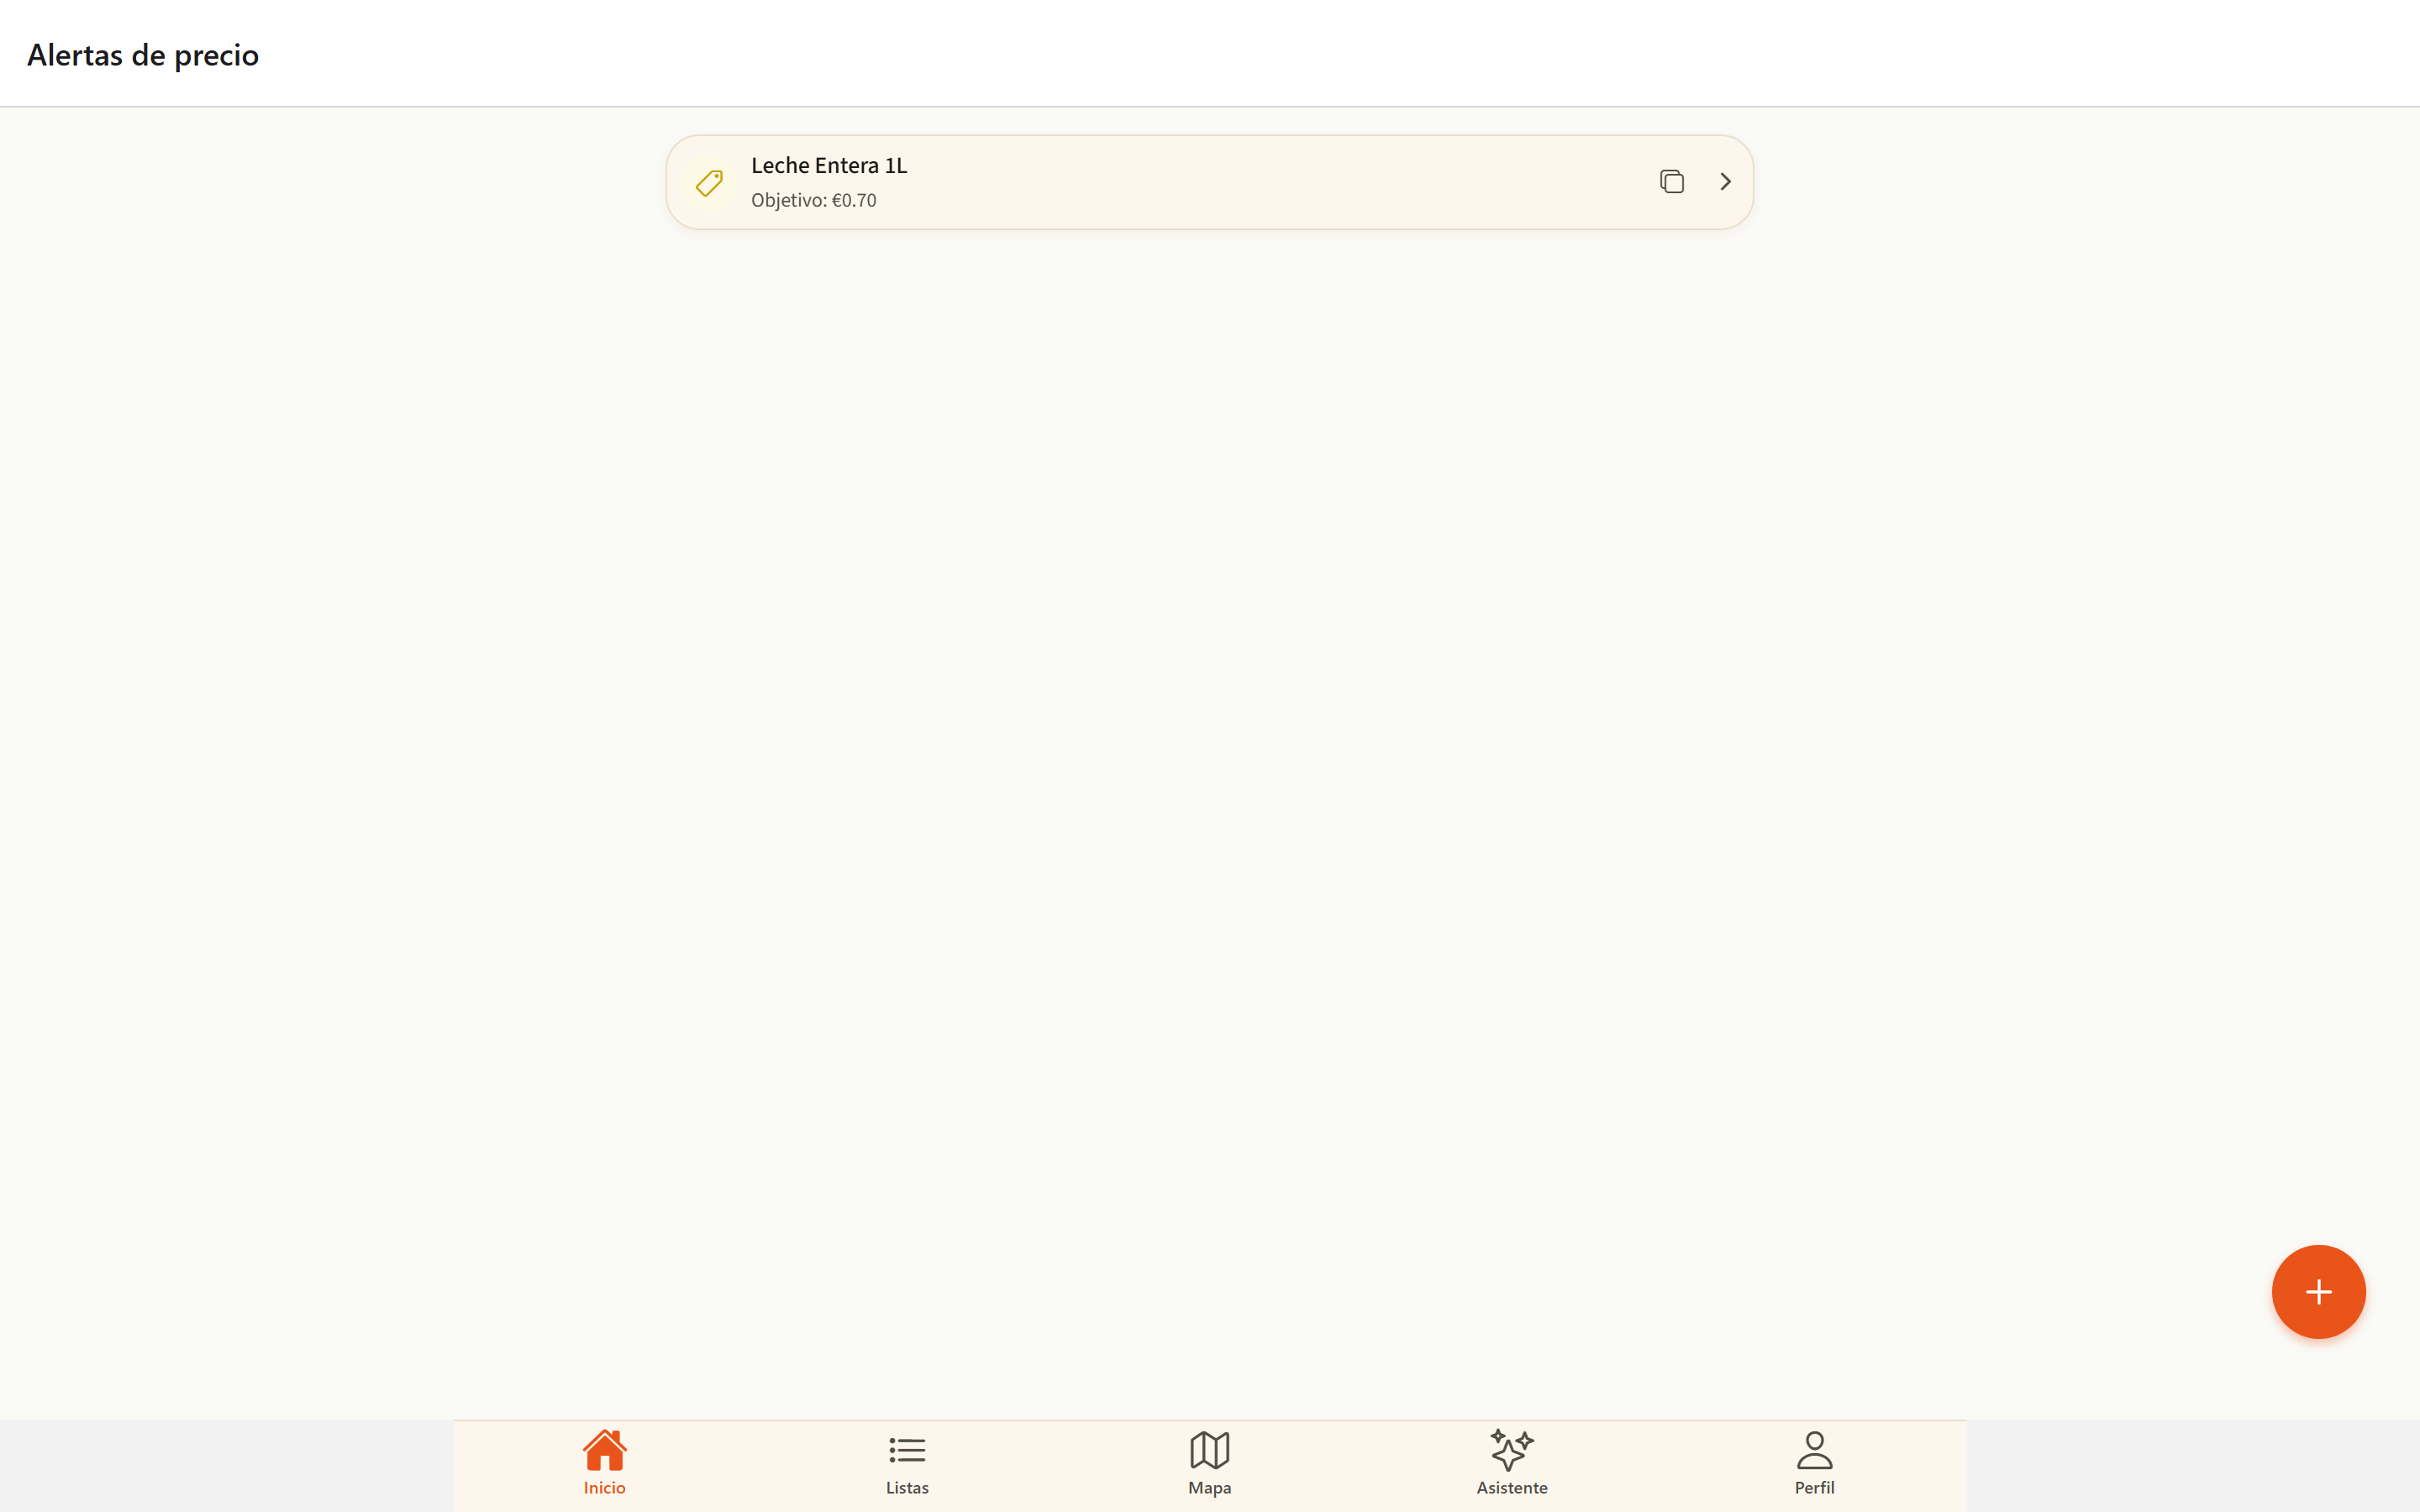
\includegraphics[width=0.48\textwidth]{diagramas/capturas/web-alertas.png}
\caption{Bandeja de notificaciones (izquierda) y alertas de precio (derecha) en la versión de
escritorio}
\label{fig:manual-web-notifs}
\end{figure}
